% !Mode:: "TeX:UTF-8"
%% 请使用 XeLaTeX 编译本文.
% \documentclass{WHUBachelor}% 选项 forprint: 交付打印时添加, 避免彩色链接字迹打印偏淡. 即使用下一行:
\documentclass[forprint]{OSPaper}
\usepackage{listings}
\usepackage{xcolor}

\lstset{
	language=python,  %代码语言使用的是matlab
	frame=shadowbox, %把代码用带有阴影的框圈起来
	rulesepcolor=\color{red!20!green!20!blue!20},%代码块边框为淡青色
	keywordstyle=\color{blue!90}\bfseries, %代码关键字的颜色为蓝色,粗体
	commentstyle=\color{red!10!green!70}\textit,    % 设置代码注释的颜色
	showstringspaces=false,%不显示代码字符串中间的空格标记
	numbers=left, % 显示行号
	numberstyle=\tiny,    % 行号字体
	stringstyle=\ttfamily, % 代码字符串的特殊格式
	breaklines=true, %对过长的代码自动换行
	extendedchars=false,  %解决代码跨页时,章节标题,页眉等汉字不显示的问题
	%   escapebegin=\begin{CJK*},escapeend=\end{CJK*},      % 代码中出现中文必须加上,否则报错
	texcl=true}

\begin{document}

%%%%%%% 下面的内容, 据实填空.

\miji{ }                                      % 密级. 没有就空着.
\StudentNumber{202010311229} % 填写自己的学号

\title{操作系统课程设计\\网络聊天室}
\Etitle{Operation System Course Design} % 英文题目
\author{孙思进}                            % 作者名字
\Eauthor{Sijin Sun}            %作者英文名
\Csupervisor{毕坤\quad 老师}        %指导教师中文名、职称
\Esupervisor{Teacher Kun Bi}     %指导教师英文名、职称
\Cmajor{计算机科学与技术}                  % 专业中文名
\Emajor{Computer Science and Technology}% 专业英文名
\Cschoolname{信息工程学院}          % 学院名
\Eschoolname{College of Information Engineering} %学院英文名. 不确定的话, 请看一下自己学院的网页上是怎么写的. 别搞错了!
\date{二〇二一年十一月}                    % 日期, 要注意和英文日期一致!!
\Edate{October, 2021}                       % 英文封面日期

%-----------------------------------------------------------------------------
\pdfbookmark[0]{封面}{title}         % 封面页加到 pdf 书签
\maketitle
\frontmatter
\pagenumbering{Roman}              % 正文之前的页码用大写罗马字母编号.
%-----------------------------------------------------------------------------
% !Mode:: "TeX:UTF-8"
\thispagestyle{empty}
\renewcommand{\baselinestretch}{1.5}  %下文的行距

\begin{cnabstract}
本报告介绍了操作系统课程设计作品:《网络聊天室》的原理组成。本软件通过$Pythony$语言编写,
使用$ Socket $通信的方式,实现了点对点、点对面的文本信息传递功能,巧妙利用$ FTP $服务器的功能实现了图片
传输、视频传输、音频传输等功能。最终的成品运行在阿里云主机上,实现真正意义上的网络聊天功能。



\end{cnabstract}
\par
\vspace*{2em}

\cnkeywords{操作系统; 网络聊天室; $ socket $; $ C\&S $ }
\\
\enkeywords{Operation System;Internet Chat; socket;C\&S}
    % 加入摘要, 申明.
%==========================把目录加入到书签==============================%%%%%%
\pdfbookmark[0]{目录}{toc}
\tableofcontents
\mainmatter %% 以下是正文
%%%%%%%%%%%%%%%%%%%%%%%%%%%--------main matter-------%%%%%%%%%%%%%%%%%%%%%%%%%%%%%%%%%%%%
\chapter{引言}
\section{动机}
二零二一年正是$ 5G $通信的商用元年,回顾初代互联网的诞生,通信方式改善了人们的生活,从最初的短信单向通信,到$ Microsoft \; MSN$ ,从$ Xiaomi \;$ 米聊,到 $Tencent \; QQ $,再到$Tencent \; WeChat$,大大提高了人们的沟通方式。

\begin{figure}[ht]
	\centering
	\begin{minipage}[t]{0.33\linewidth}
		\centering
		
\includegraphics{msn.jpg}
		\caption{$MSN \;$中国}
		\label{fig:1}
	\end{minipage}%
	\begin{minipage}[t]{0.33\linewidth}
		\centering
		
\includegraphics{qq.jpg}
		\caption{$Tencent \; QQ $}
		\label{fig:2}
	\end{minipage}%
	\begin{minipage}[t]{0.33\linewidth}
		\centering
		
\includegraphics{wechat.jpg}
		\caption{$Tencent \; WeChat $}
		\label{fig:3}
	\end{minipage}%
\end{figure}

笔者设想编写一个基于互联网传输的网络聊天室,用于点对点通信和多对多通信的交流。

为了提高沟通效率,方便人们及时获取信息,本文设计并完成了一个网络聊天室系统,采用$  C/S  $模式,在$ Pycharm \; Python3.7 $环境下结合$ Neo4j $数据库技术进行设计。

\section{要解决的问题}

编写一个网络聊天室,对于服务器来说,需要做到如下几个功能:

\begin{itemize}
	\item 直接
	\item 快速
	\item 低延迟
	\item 安装便捷
	\item 多媒体化
\end{itemize}

\subsection{通信方式}
涉及到点对点通信,$socket$的通信方式显然是首要选择方式,它基于$TCP/IP$协议,实现了点对点的通信,并且传输速度不受其他因素限制。由于采用嵌套字传输方式,在安全方面可能存在一定风险,有被抓包分析的可能性。

对于私人和多人聊天有着不同的功能要求,私人聊天之间需要较高的加密程度,确保信息安全;而多人公开聊天中,则需要考虑多并发的情况,对于一个消息文本,短时间瞬发需求极大,软件需要保证不漏发、不错发的前提下高效率的传输信息。
\begin{figure}[ht]
	\centering
	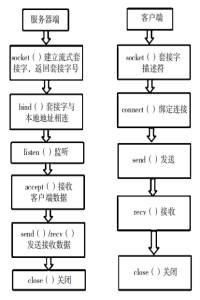
\includegraphics{tongxin.jpg}
	\caption{通信原理\upcite{r1}}
	\label{fig:4}
	
\end{figure}

\subsection{架构方式}
为了做到高效的通信,减少用户端设备的硬件要求,本软件采用$ C/S $端的假设方式,$ C $端即为$ Client $:客户端,$ S $端即为$ Serve $:服务器端。

本软件初代运行在局域网中,将服务器端假设在局域网的某台电脑中,实现了群聊和单聊的通信功能。考虑到在一定程度上无法每时每刻连接内网的网关,故后续将本软件的服务器端架设在阿里云上,实现了广域网通信。


客户端/服务器模型最终归结为一个“请求/应答”的关系。一个请求总是第一个颁发给客户端,然后服务器总是被动地接收请求,返回结果给客户需要。在客户端发送一个请求时,服务过程一直处于休眠状态。在一个客户端请求时,服务过程是“唤醒”和为客户提供服务,根据客户的要求进行回复。\upcite{r2}因此采用socket框架。

\subsection{编程语言选择}

本软件使用$ Python $语言开发,不涉及库文件的安装情况下,编译打包前的源文件不到1mb,并且python的同一个代码源文件可以同时在$Linux \; MacOS \; Windows$系统运行,实现了轻量化的设计需求。

使用的库如表\ref{table:1}所示
\begin{table}[ht]\centering
	\caption{$Python$配置包}
	\label{table:1}
	\begin{tabular}{ccl}
		\hline
		序号 & 名称       & 功能                           \\ \hline
		1  & $Socket$    & 实现点对点通信                   \\
		2  & $Tkinter$   & 图形化$GUI$                      \\
		3  & $openCV$    & 显示图片、视频、音频等多媒体信息    \\
		4  & $ftplib$    & 传输文件                           \\
		5  & $json$      & 打包数据,生成嵌套字                \\
		6  & $threading$ & 实现多线程                          \\
		7  & $py2neo$    & $Neo4j$在$Python \;$运行的基础库     \\ \hline
	\end{tabular}
\end{table}

\subsection{双端环境配置}

本软件的编译和运行均基于表\ref{table:2}的环境下配置,此外,设计报告撰写使用\LaTeX{}。

\begin{table}[ht]\centering
	\caption{系统环境}
	\label{table:2}
	\begin{tabular}{ccl}
		\hline
		序号 & 名称        & 版本                                                        \\ \hline
		1  & 客户端       & $Windows \;10 \; Professior$                              \\
		2  & 服务器端      & $Windows \; 10 \; DataBase $\\
		3  & $PyCharm$ & $PyCharm \; Community \; 2021.2.2$                        \\
		4  & $Java$    & $Java \; JDK \; 18$                                       \\
		5  & \LaTeX{}   & $TexLive \; 2020$                                      \\
		6  & $Neo4j$   & $Neo4j \; Community 4.3.5$                                \\ \hline
	\end{tabular}
\end{table}

\subsection{图形界面构建}

为实现图形界面可视化,本软件使用了$Python$内置包$Tkinter$来构建用户界面。$Tkinter$有着所见即所得的称谓,通过编程按钮、功能进行布局和设计,可以减少设计的难度。

对于客户端而言,主要负责用户的登录和注册,以及最重要的收发消息。

对于服务器端而言,负责处理收到的文本,将其转发到各个用户所在的$ip$地址的端口上。

\subsection{数据库设计}

为实现通信数据的存储和用户登录信息的查询功能,数据库设计是首要的,它运用了数据模型将系统中的数据组织起来,这对系统设计而言是必不可少的。本系统设计数据库的目的是保存登录和注册时的用户信息,以用来验证登录。

数据库使用了$ Neo4j $,一种基于离散数学中图论原理的轻量数据库,普遍被称为知识图谱,相比较传统的$MySql$、$SqlLite$而言,其基本的结构由节点($Node$)、关系($Relationship$)和标签($Label$)组成,通过这三个属性可以构建出传统数据库没有的功能。

如图\ref{fig:10}所示,源文件为一个有关于心理测试的调查信息,通过简单的$NLP$处理后,可以将原来的字段拆分成多个关系,形成有向关系网路。

\begin{figure}[ht]
	\centering
	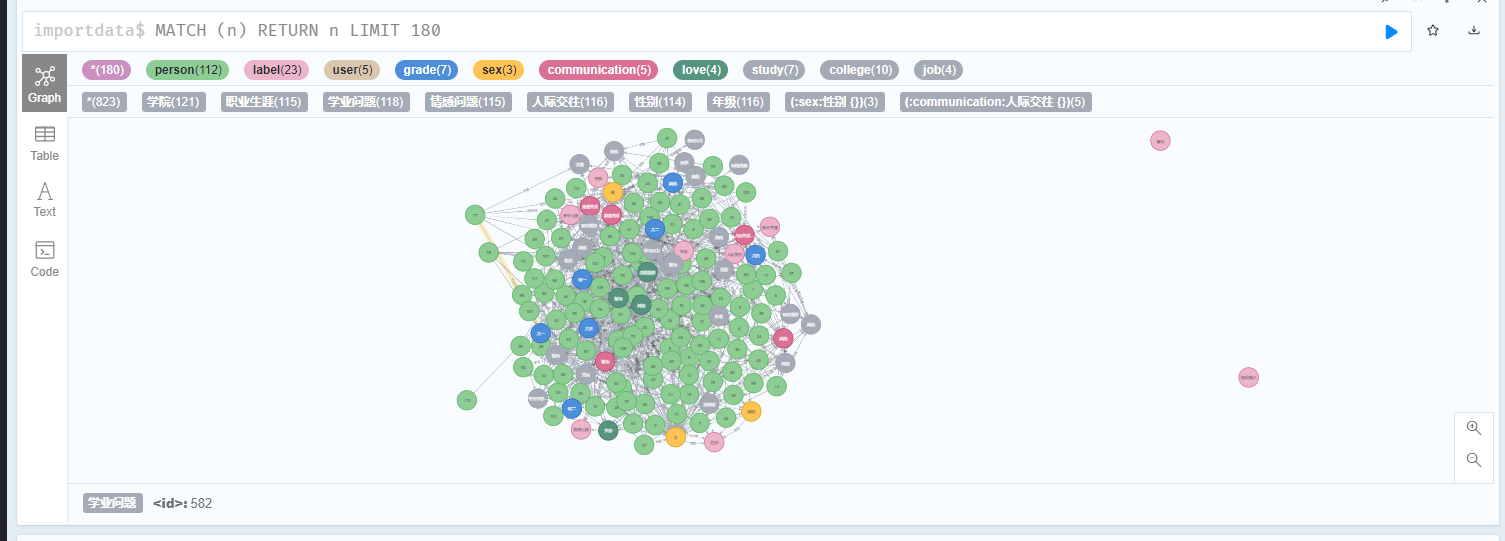
\includegraphics[width=\textwidth]{neo4j.png}
	\caption{通过$ Neo4j $形成的复杂关系图}
	\label{fig:10}
\end{figure}

此外,$Neo4j$可以储存的数据极为庞大,如\ref{table:2}所示,对于一个网络聊天室来说足矣。

\begin{table}[ht]\centering
	\caption{$Neo4j$数据容纳量}
	\label{table:3}
	\begin{tabular}{ccc}
		\hline
		S.No & 构建基块 & 数量      \\ \hline
		1    & 节  点 & 约 350 亿 \\
		2    & 关  系 & 约 350 亿 \\
		3    & 标  签 & 约 275 亿 \\ \hline
		
	\end{tabular}
\end{table}
\clearpage
\chapter{系统设计}
\section{系统总体框架}
如图\ref{fig:5}所示,整个软件的功能主要分为几个方面:

\begin{figure}[!htbp]
	\centering
	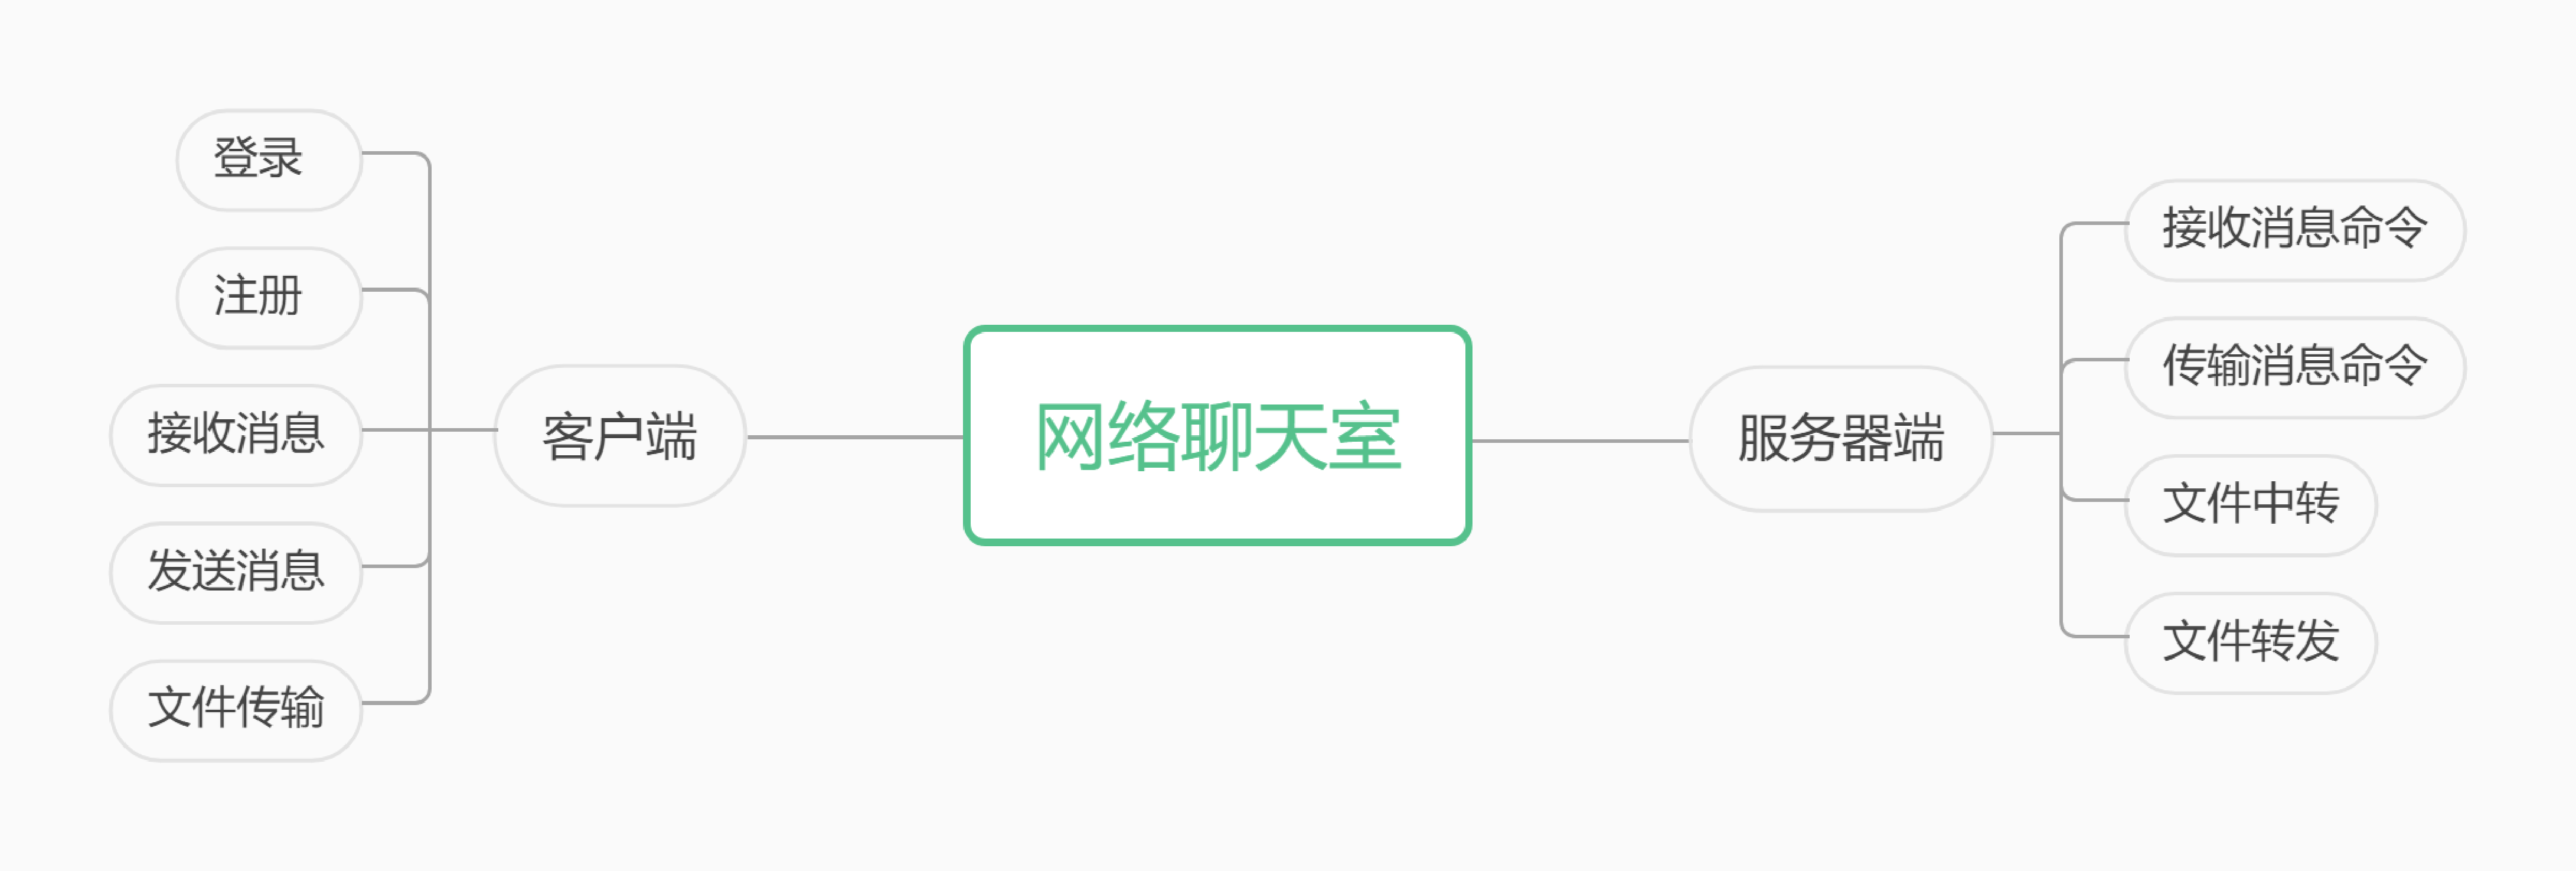
\includegraphics[width=0.7\textwidth]{chat1.pdf}
	\caption{网络聊天室框架结构}
	\label{fig:5}
\end{figure}

本软件主要由客户端和服务器端构成。客户端为用户提供了登录、注册、收发消息的功能。

服务器端提供信息收发和文件中转传输的功能。

\section{系统总体流程}

\begin{figure}[!ht]
	\centering
	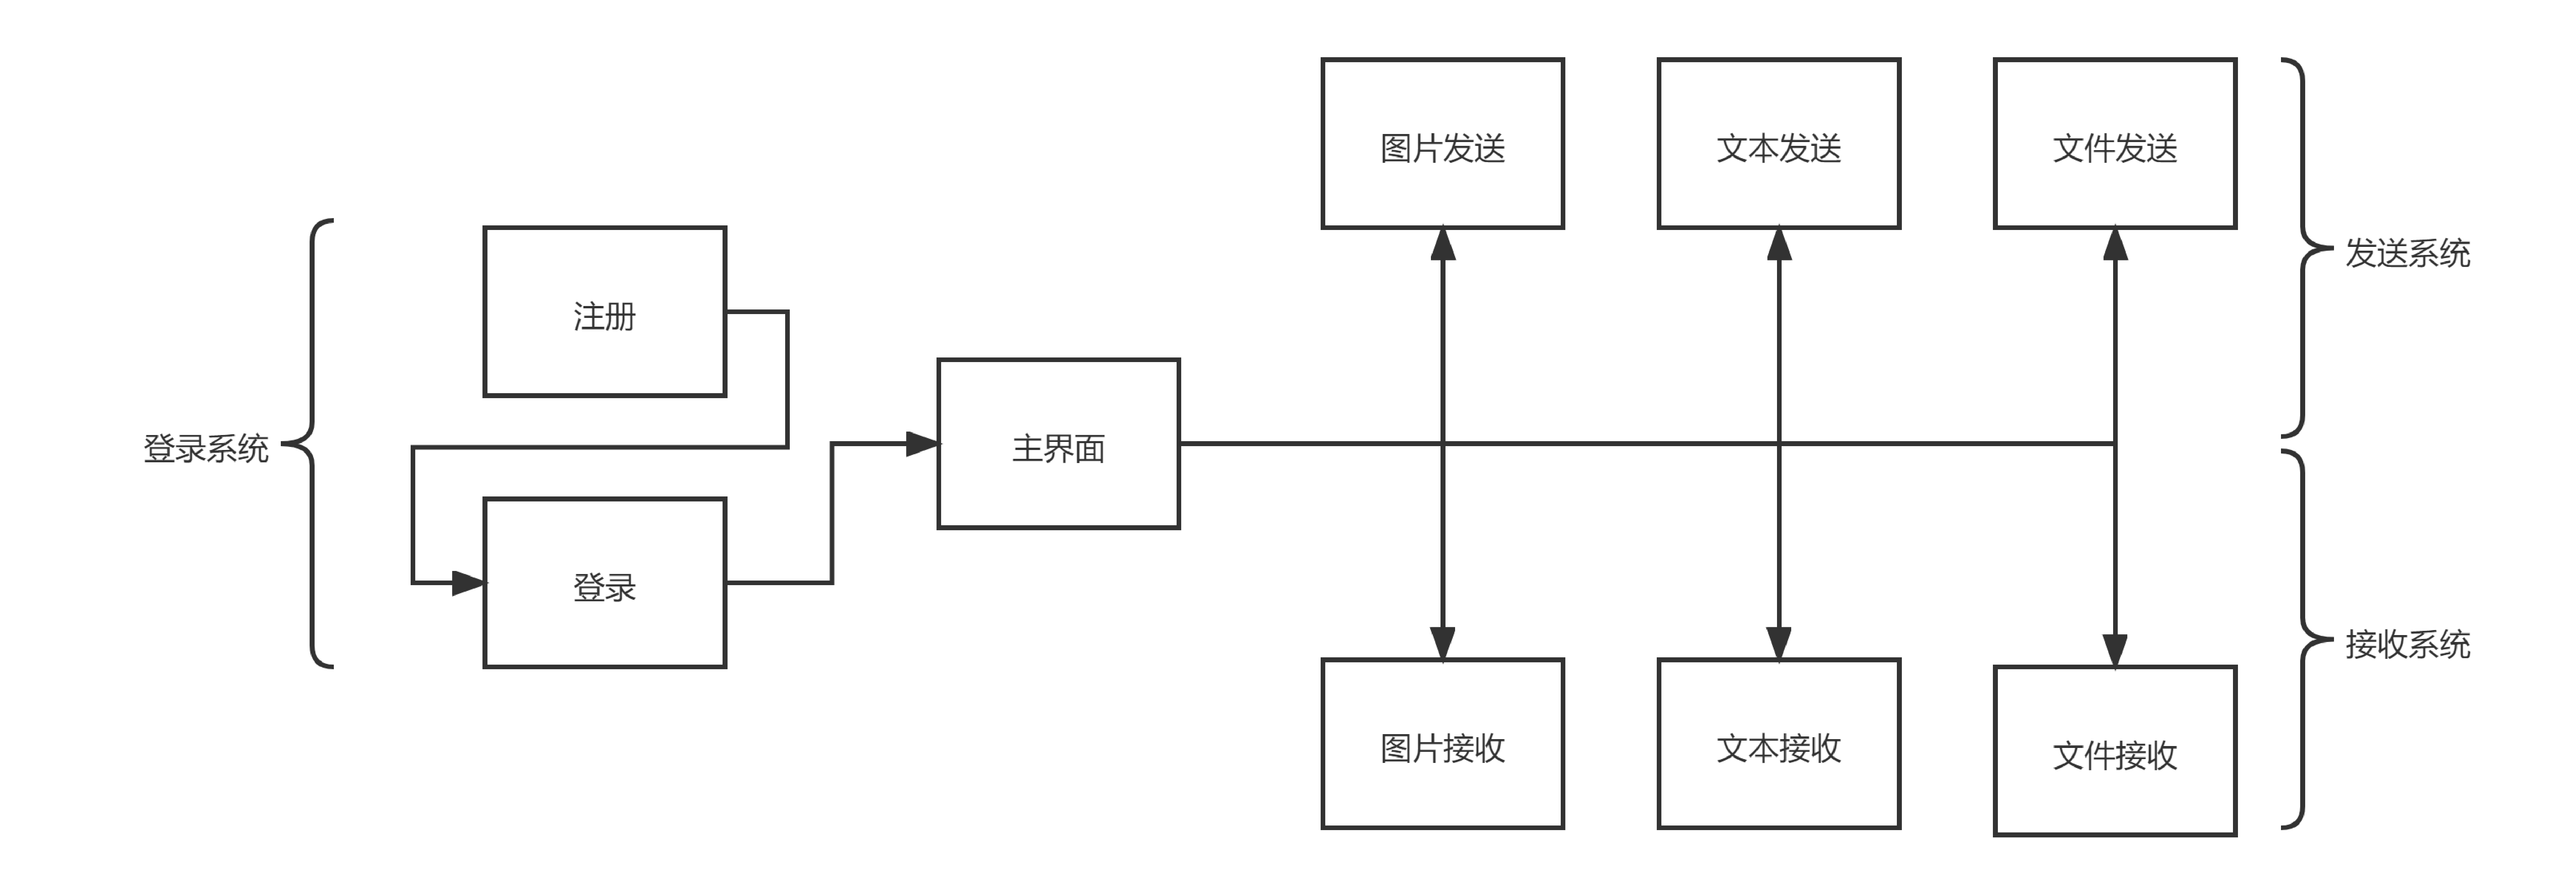
\includegraphics[width=0.7\textwidth]{system.pdf}
	\caption{网络聊天室系统流程}
	\label{fig:14}
\end{figure}

用户在登录界面,若按下注册按钮,则上传账号密码信息给服务器,服务器解析后调用数据库,若符合要求,则返回命令,提示注册成功,否通则返回注册失败;若按下登录按钮,则上传账号密码给服务器,判断账号密码是否匹配,若匹配,则登录,否则提示账号密码错误。

聊天界面提供功能有文本发送,文本接收,图片发送,图片接收功能。对于一般的图片和视频格式,都支持发送和接收。

\section{登录}
登录部分涉及到验证、确认等操作,流程如图\ref{fig:6}所示:

\begin{figure}[!ht]
	\centering
	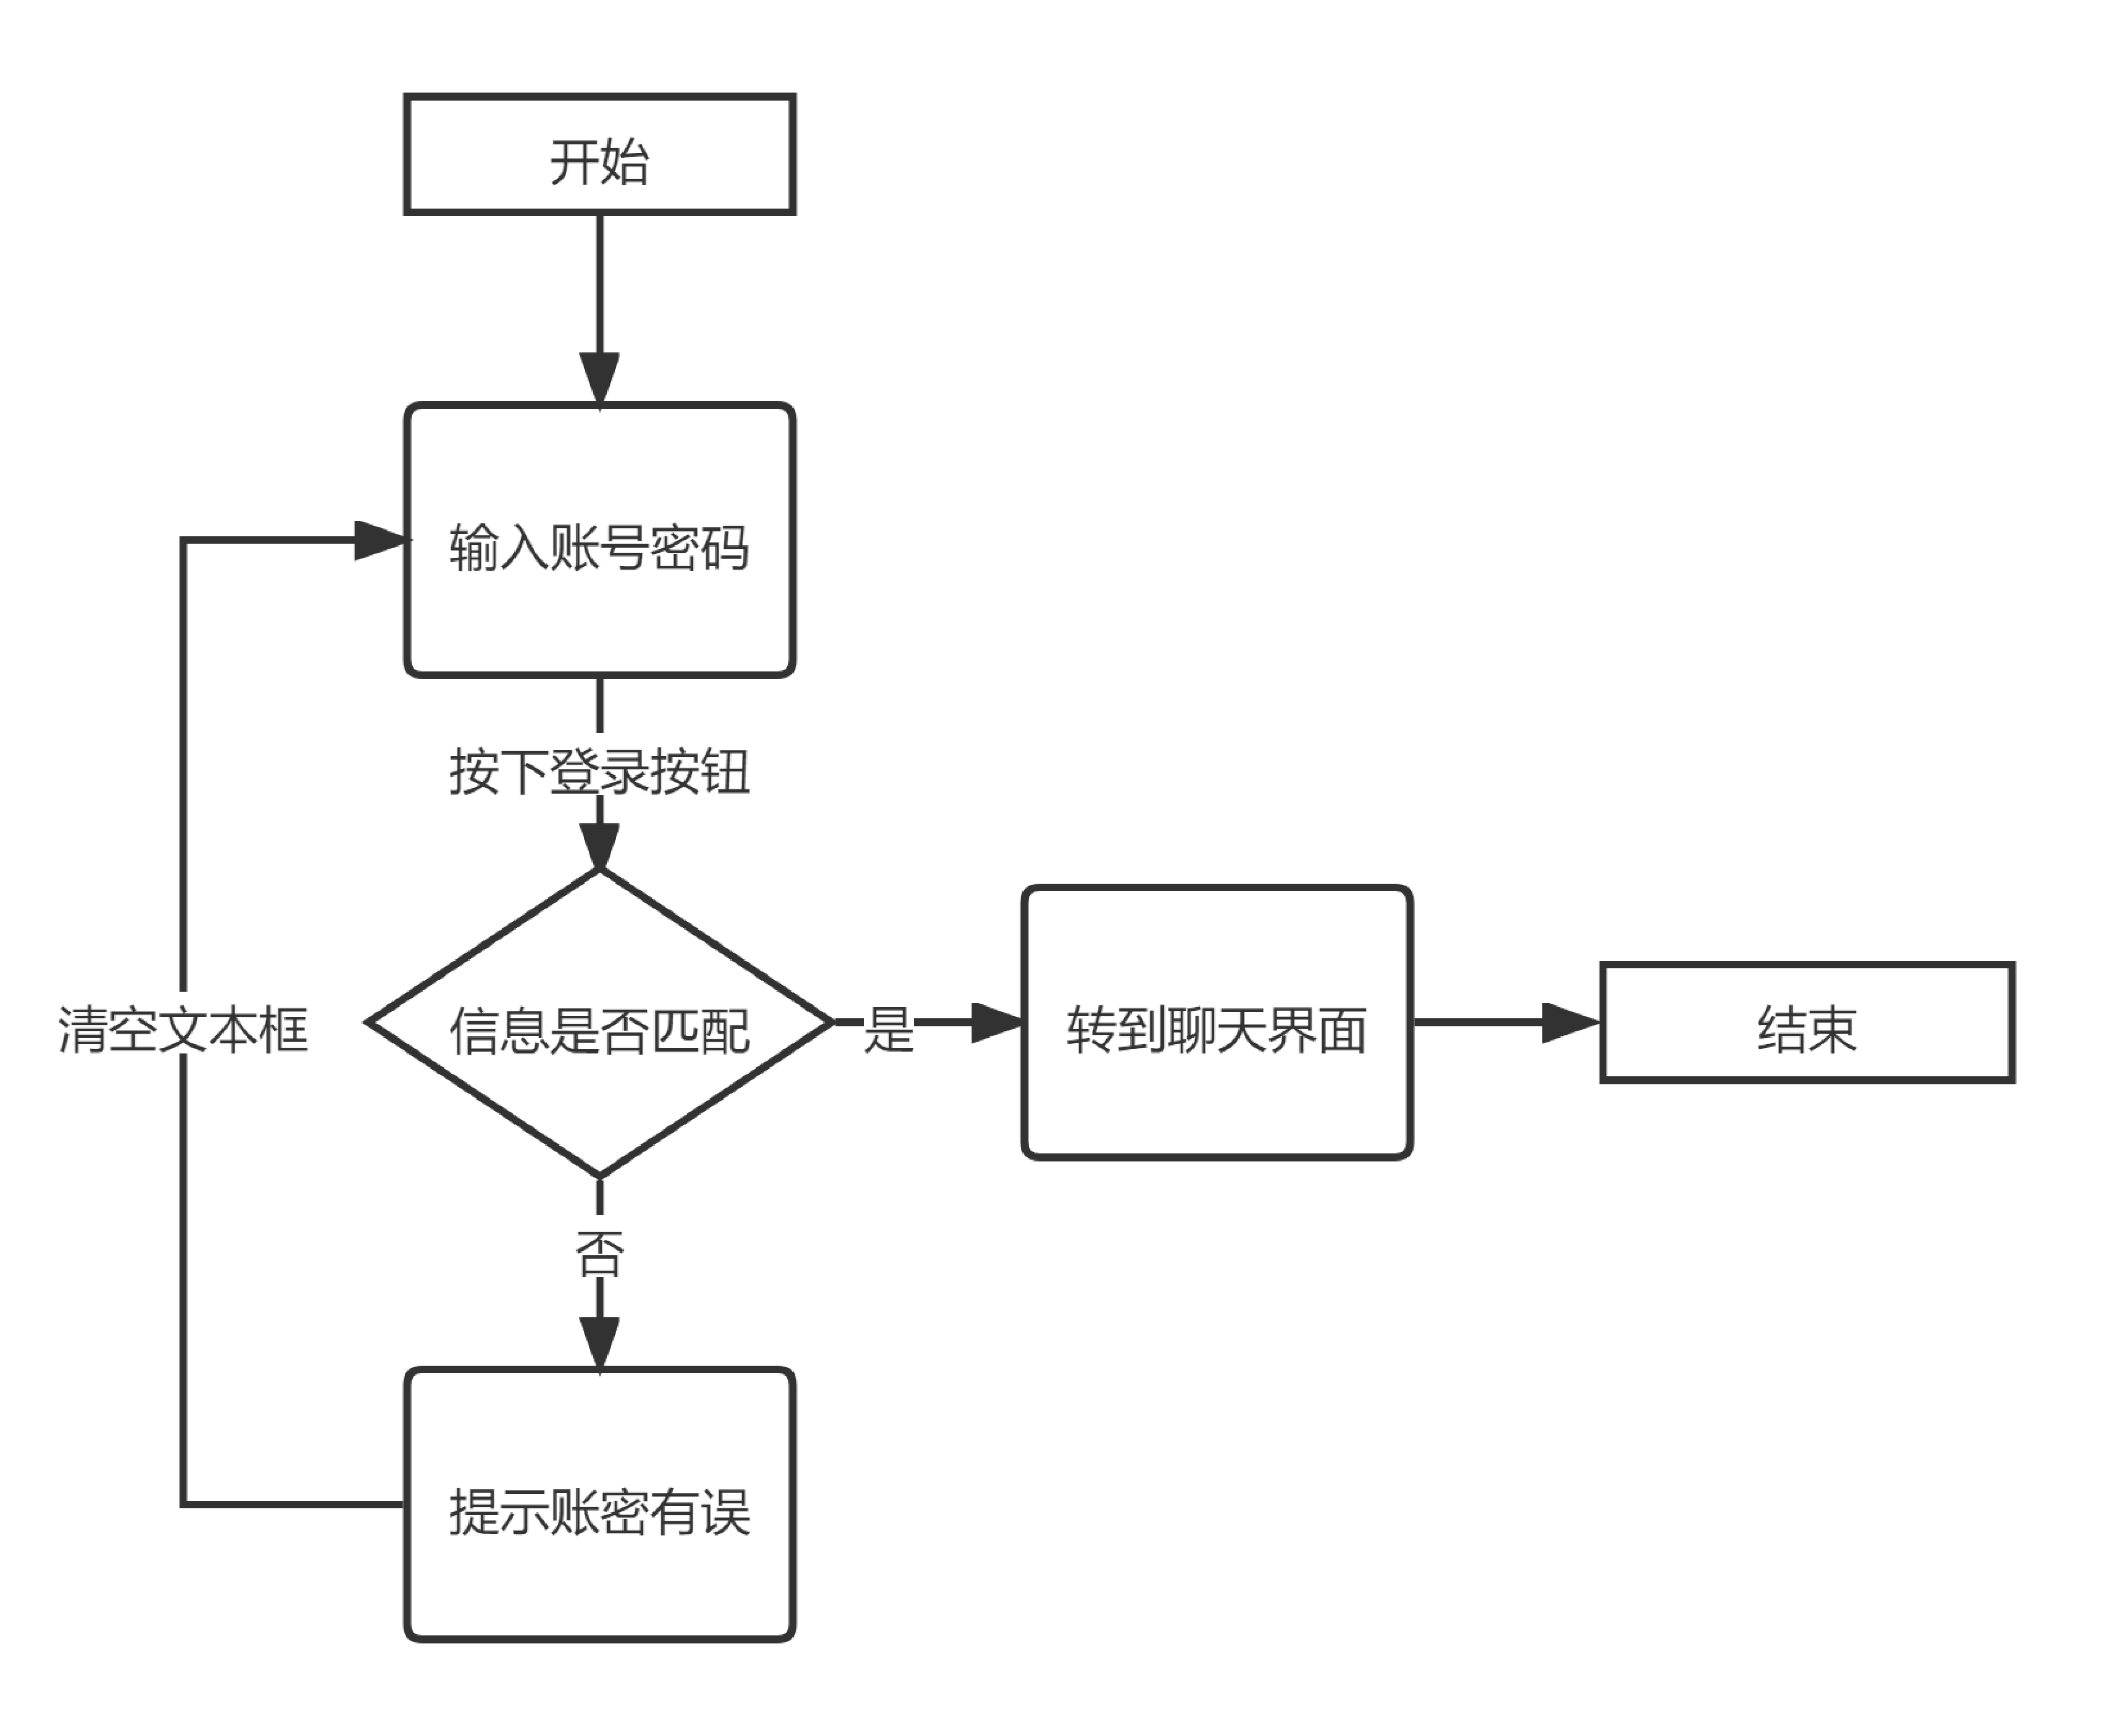
\includegraphics[width=0.4\textwidth]{login.pdf}
	\caption{登录系统流程图}
	\label{fig:6}
\end{figure}

登录时,会出现账号和密码不匹配的情况,当检测到账号密码不同时,就弹出密码错误的提升;当账号密码正确时,就进入聊天界面。

\section{注册}
使用流程图\ref{fig:7}简要的画出了注册系统的设计思路。

\begin{figure}[!htbp]
	\centering
	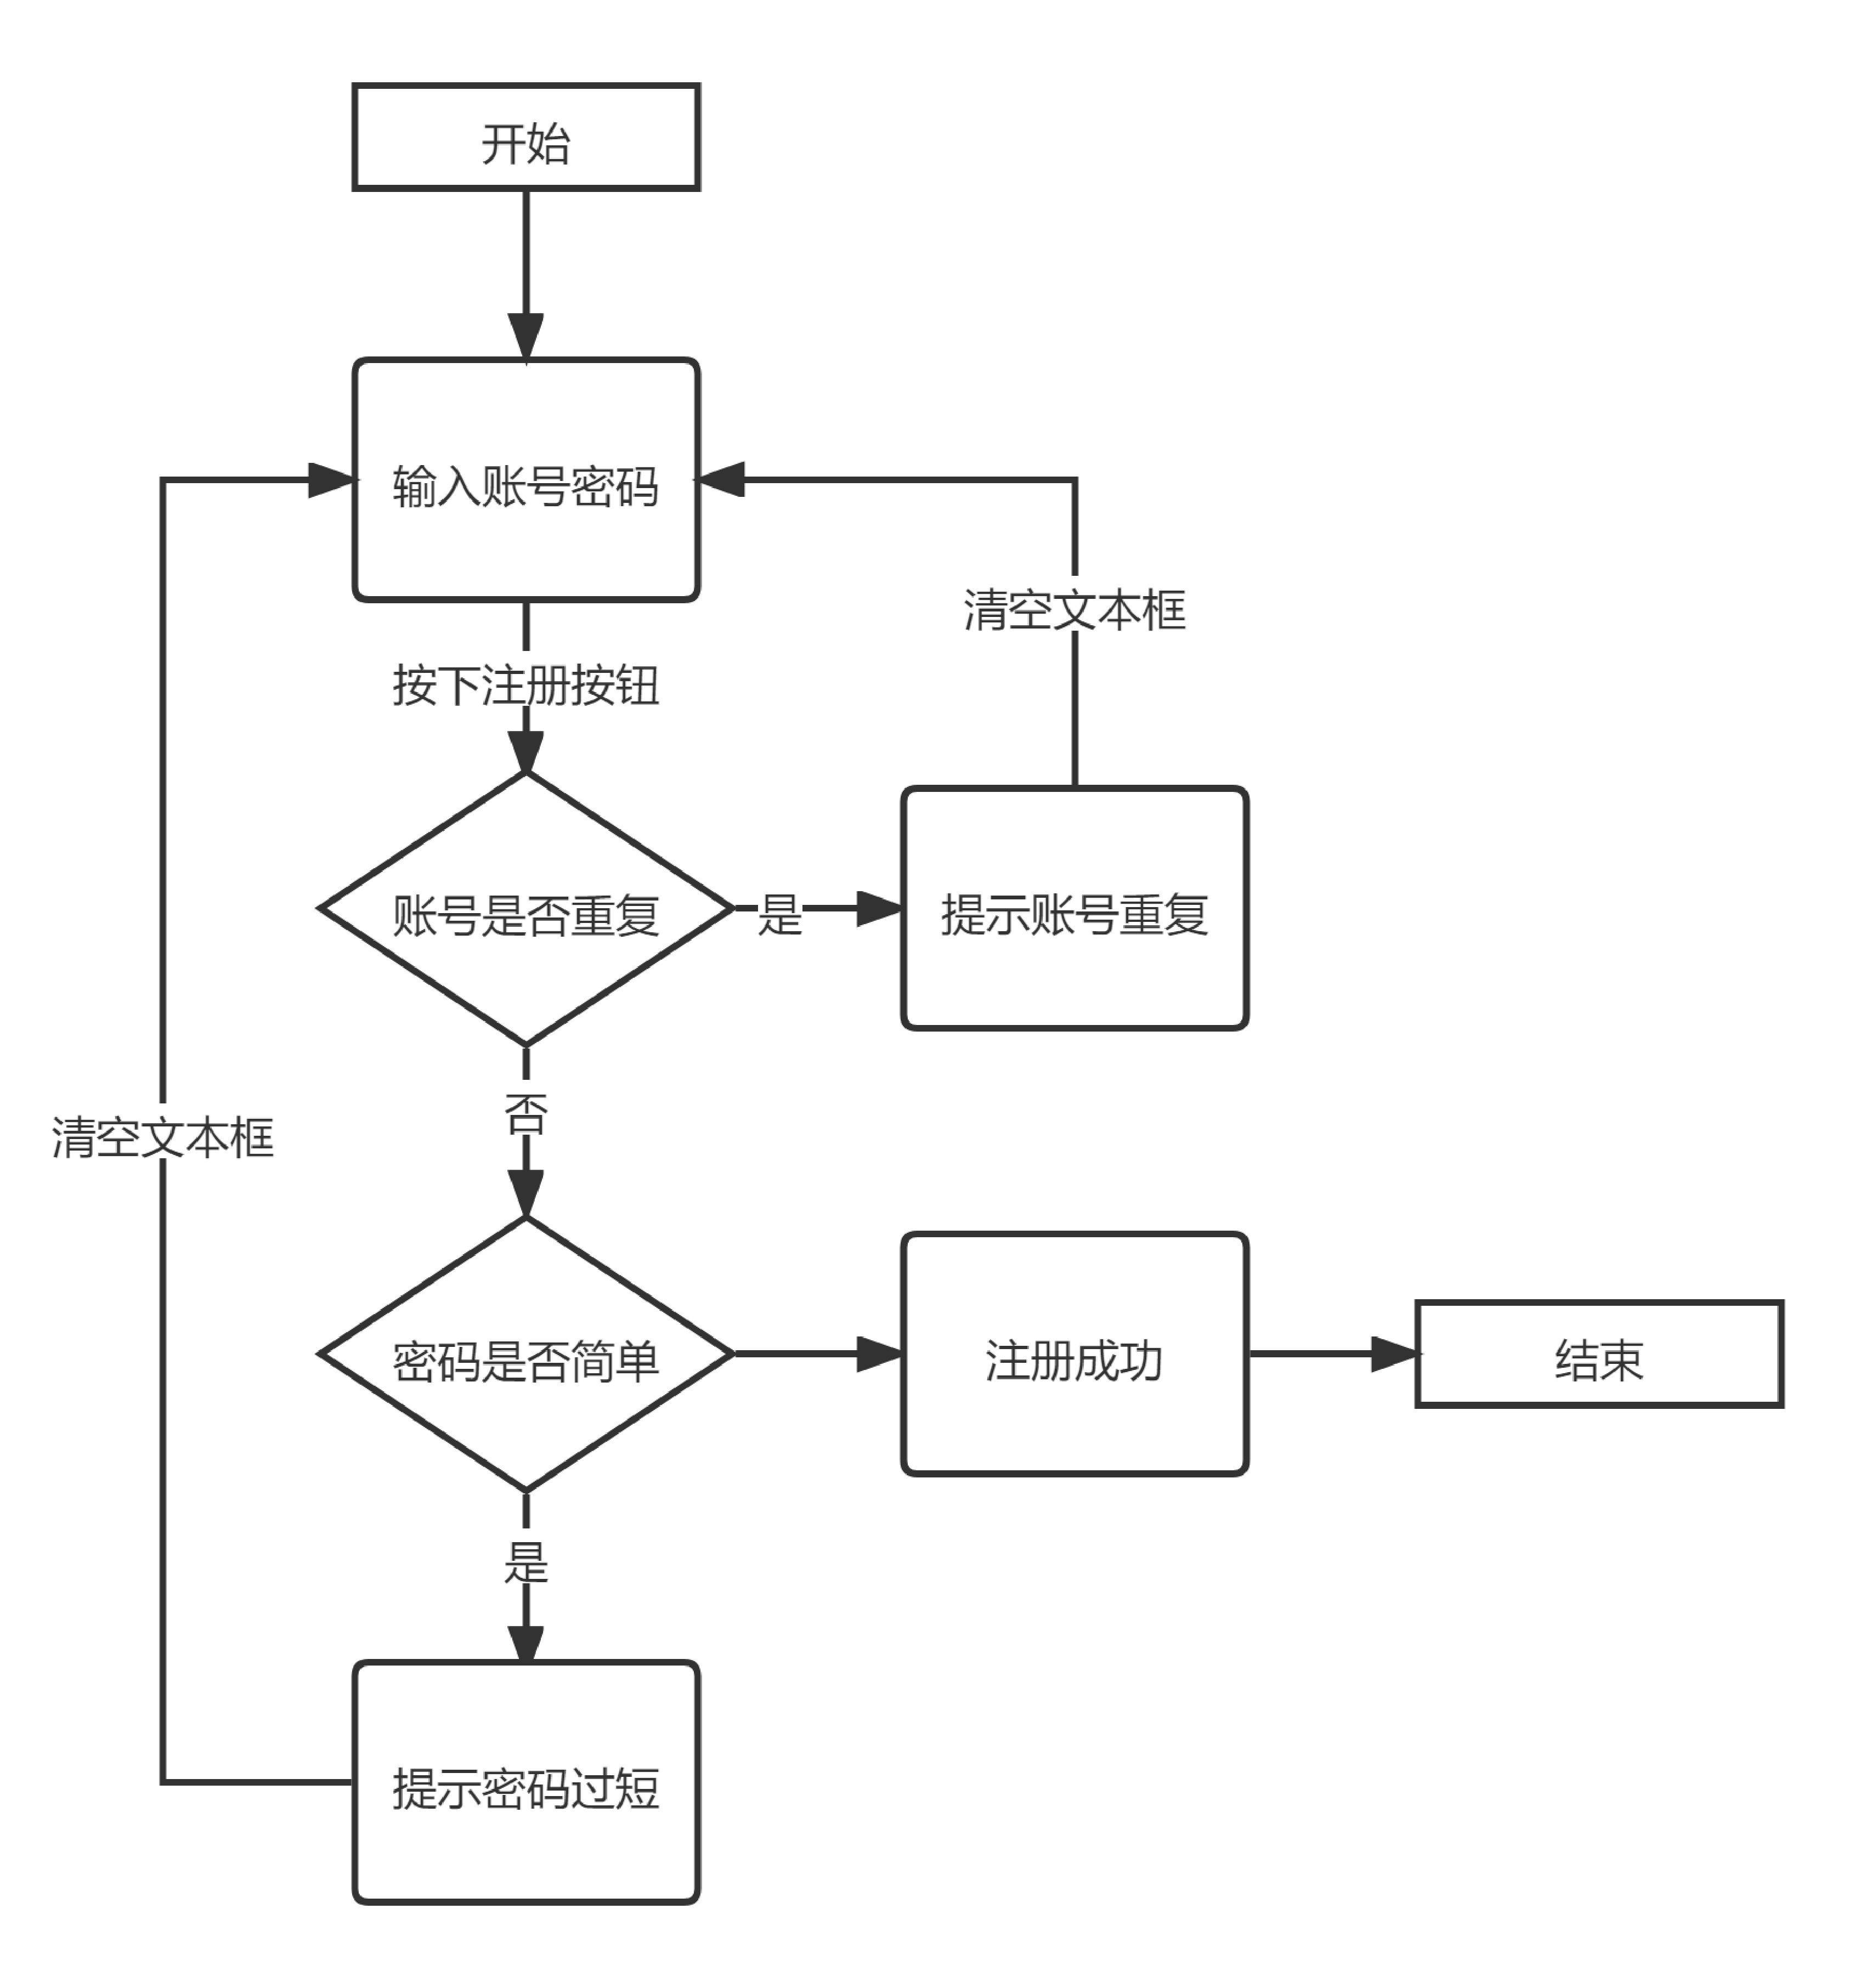
\includegraphics[width=0.5\textwidth]{regi.pdf}
	\caption{注册系统流程图}
	\label{fig:7}
\end{figure}

判定注册是否成功的标准有两个,其一是是否账号重复;其二是账号密码长度是否超过预设值(五位)。

\section{文本发送}

通过流程图\ref{fig:8}展示了文本发送的编写方法。

\begin{figure}[!htbp]
	\centering
	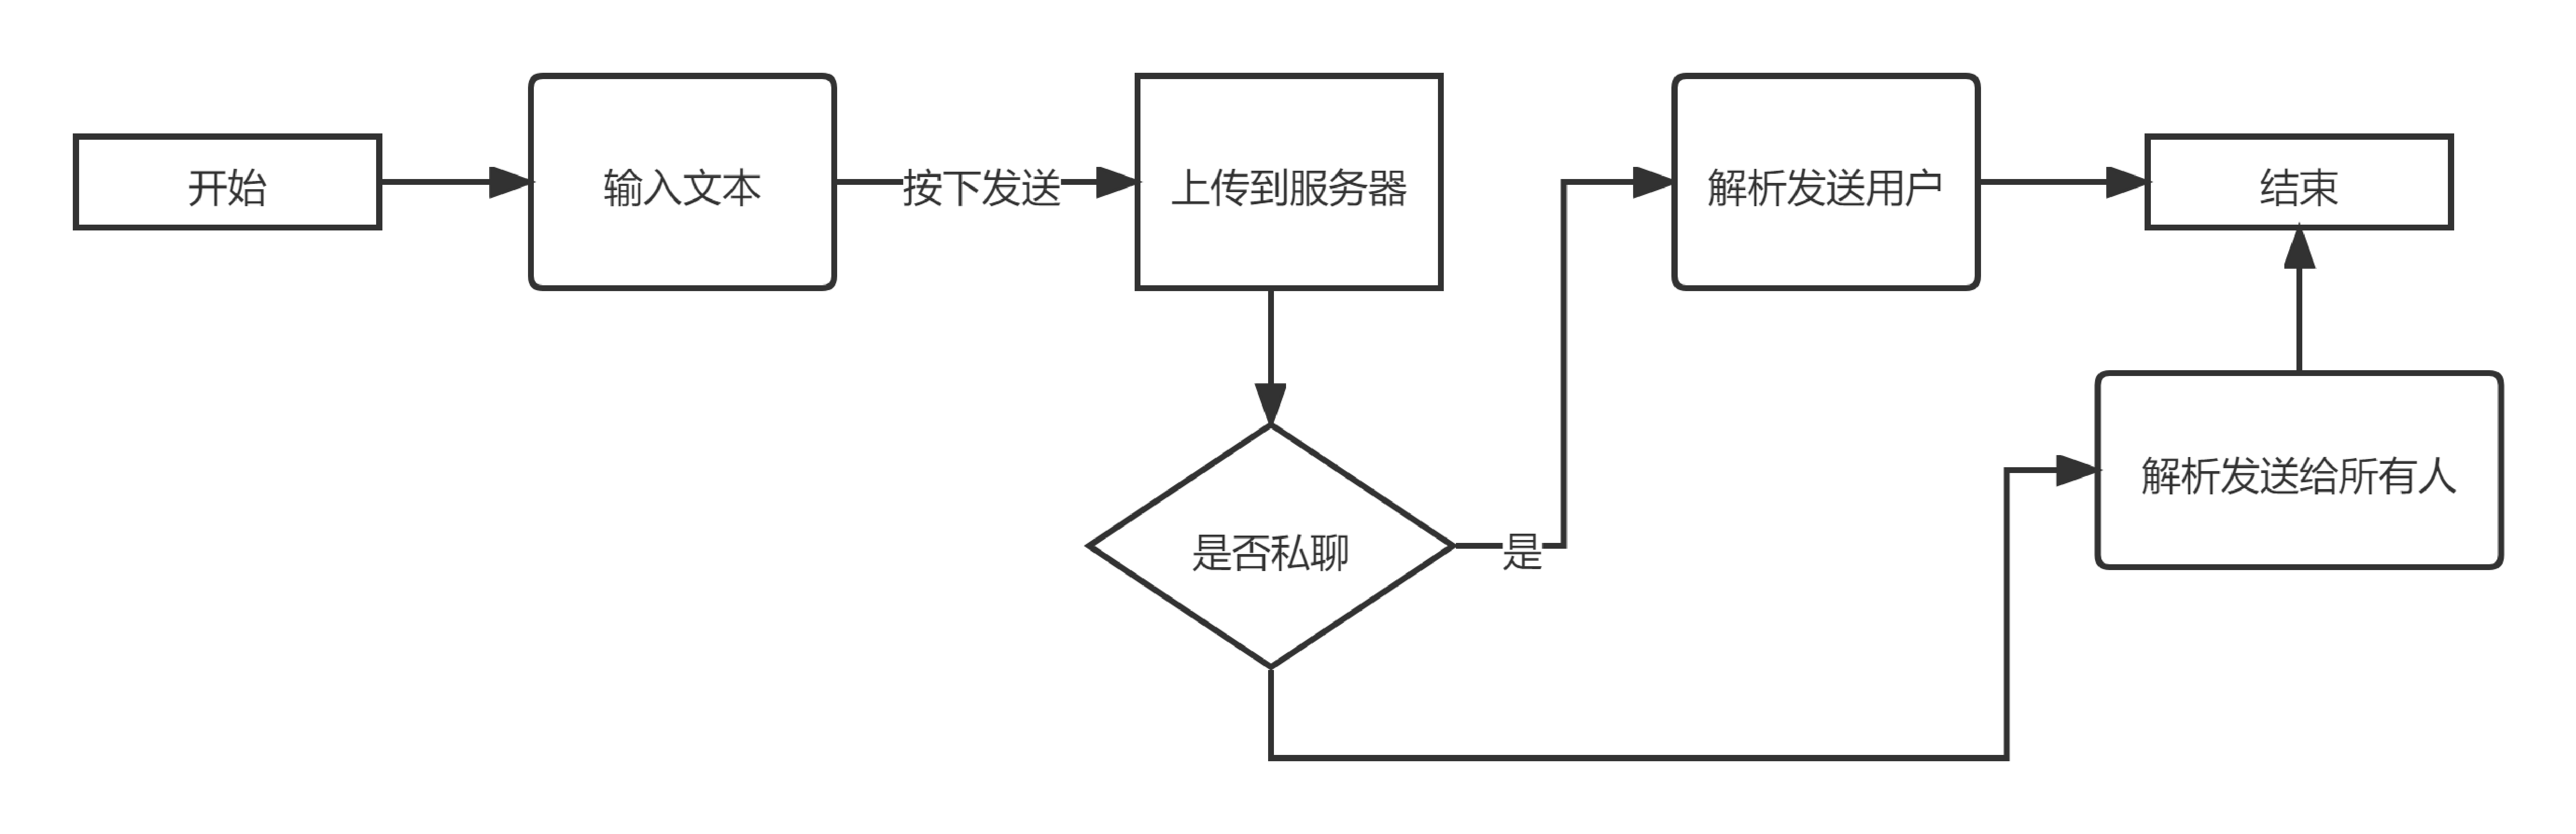
\includegraphics[width=0.6\textwidth]{text.pdf}
	\caption{文本发送流程图}
	\label{fig:8}
\end{figure}

对于文本发送,需要确认其是私聊还是群聊,确认后根据不同结果进行$ json $标注、然后再进行打包发送。

\section{文本接收}

通过流程图\ref{fig:9}展示了文本接收的编写方法。

\begin{figure}[!htbp]
	\centering
	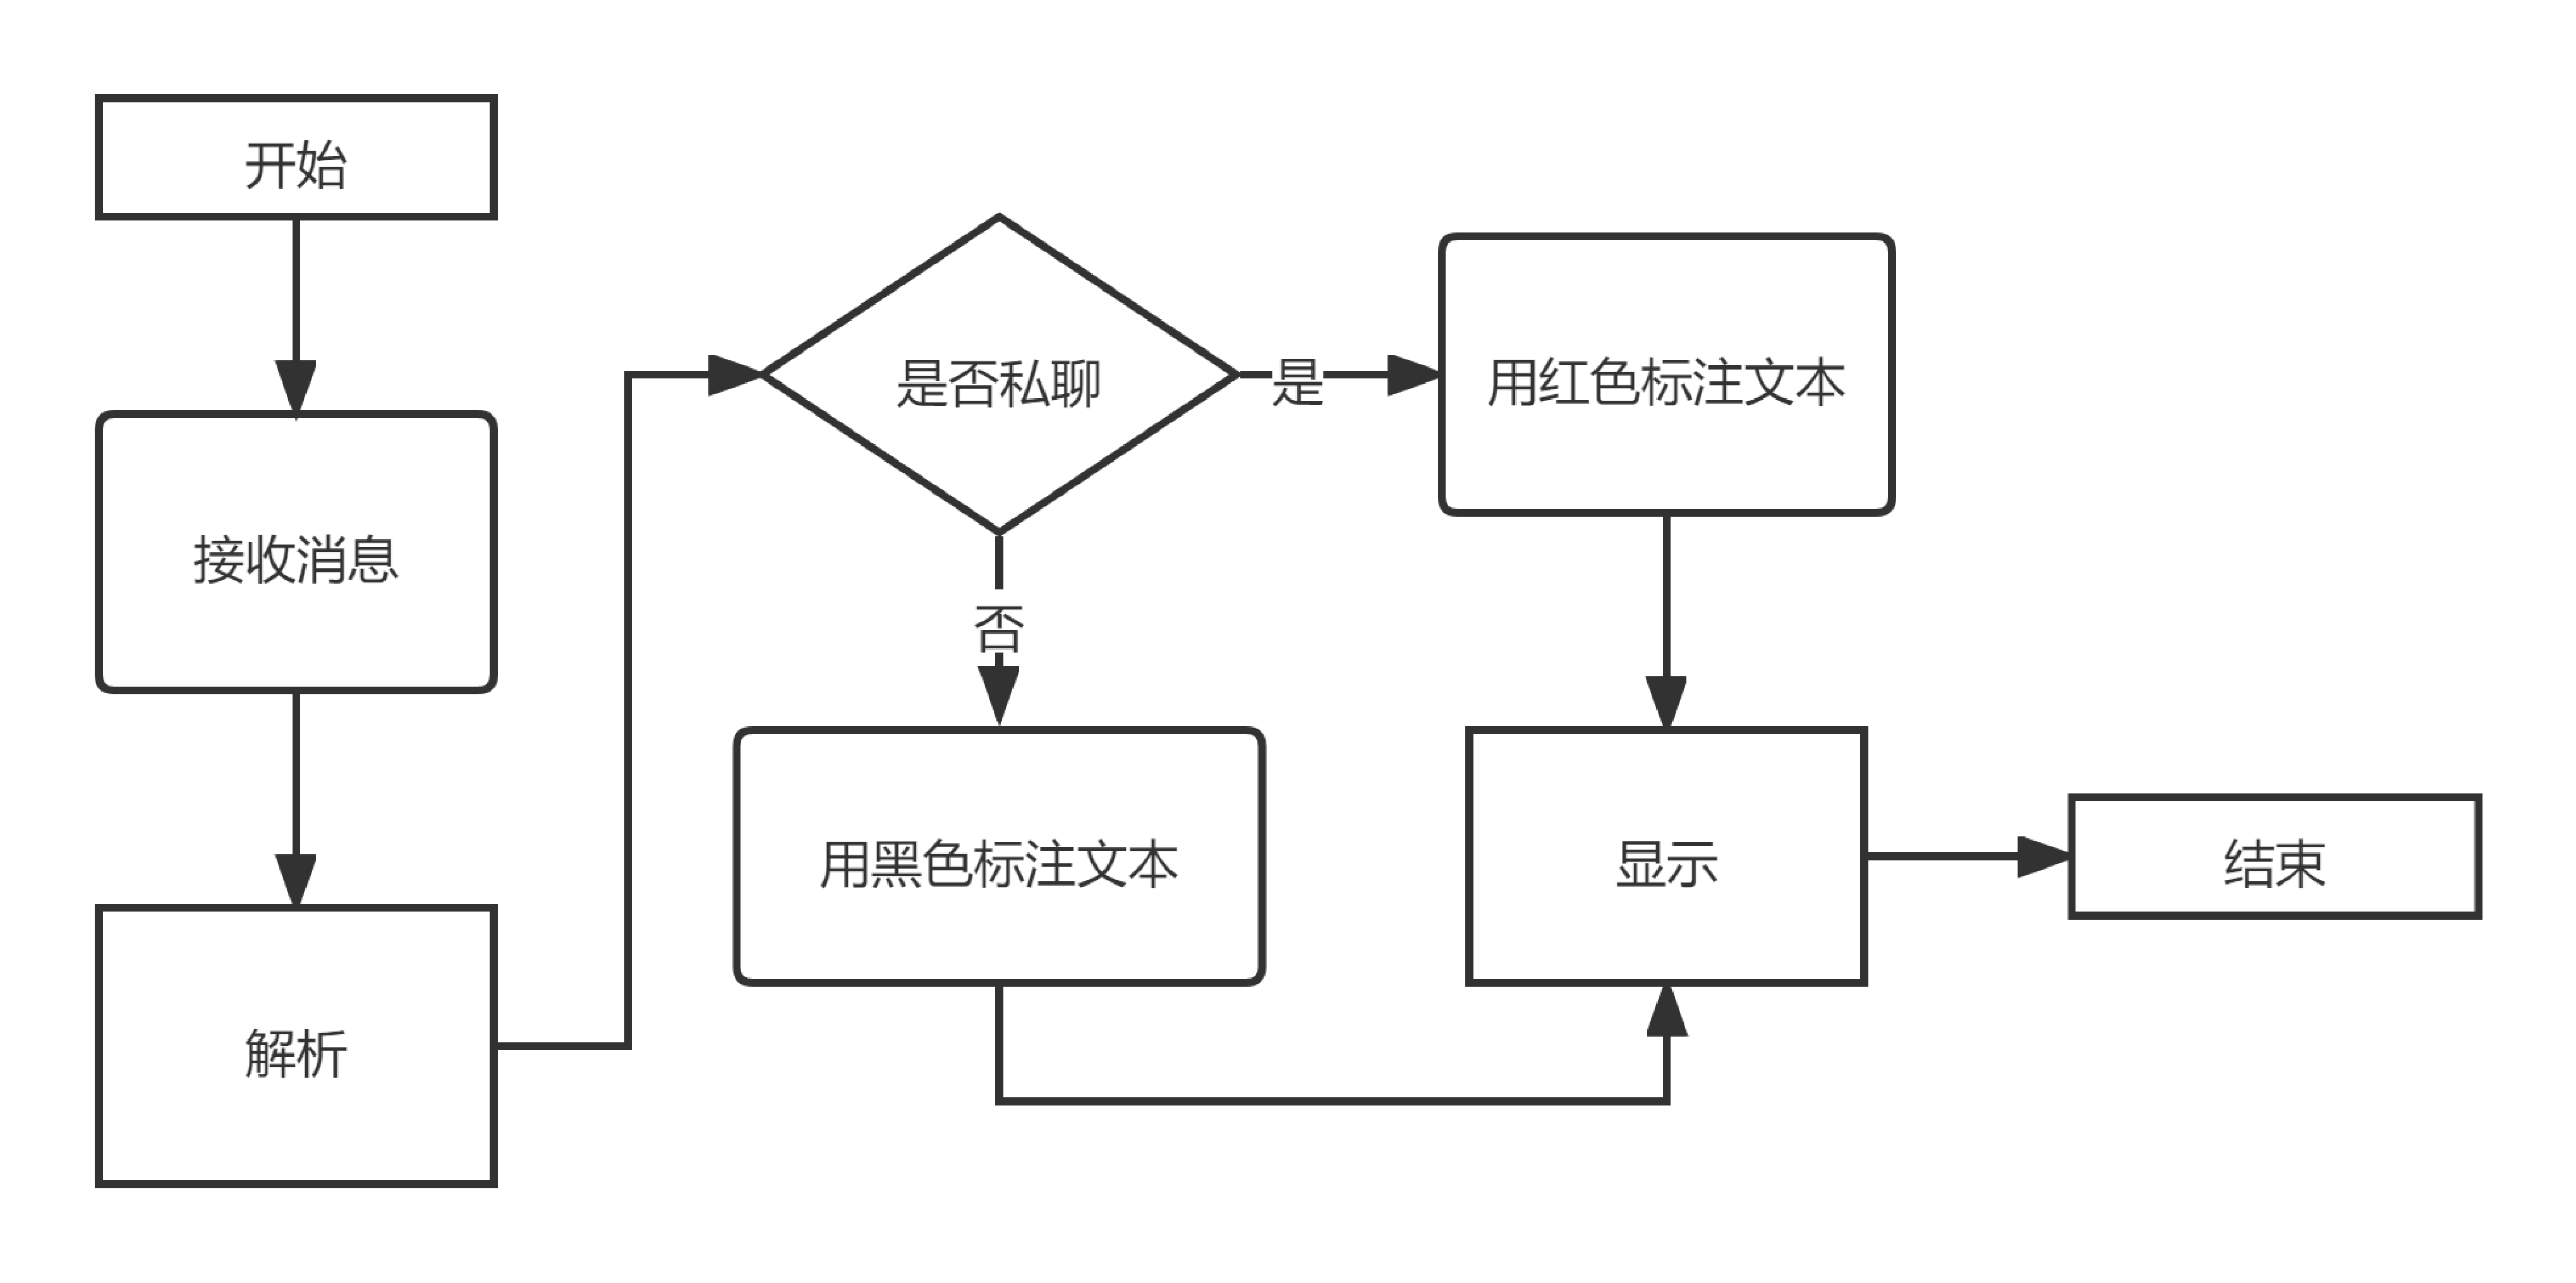
\includegraphics[width=0.8\textwidth]{receive.pdf}
	\caption{文本接收流程图}
	\label{fig:9}
\end{figure}

同样,需要考虑服务器传输的文本是群聊还是私聊,这样才能显示发送的用户,同时对不同情况下的文本进行颜色标注,以实现差异化。

\section{图片传输}
图片发送的实现运用了$FTP$服务器,间接实现了图片的传输,同时也能实现聊天记录保存的功能。如流程图\ref{fig:11}所示,图片传输的方式:

\begin{figure}[!htbp]
	\centering
	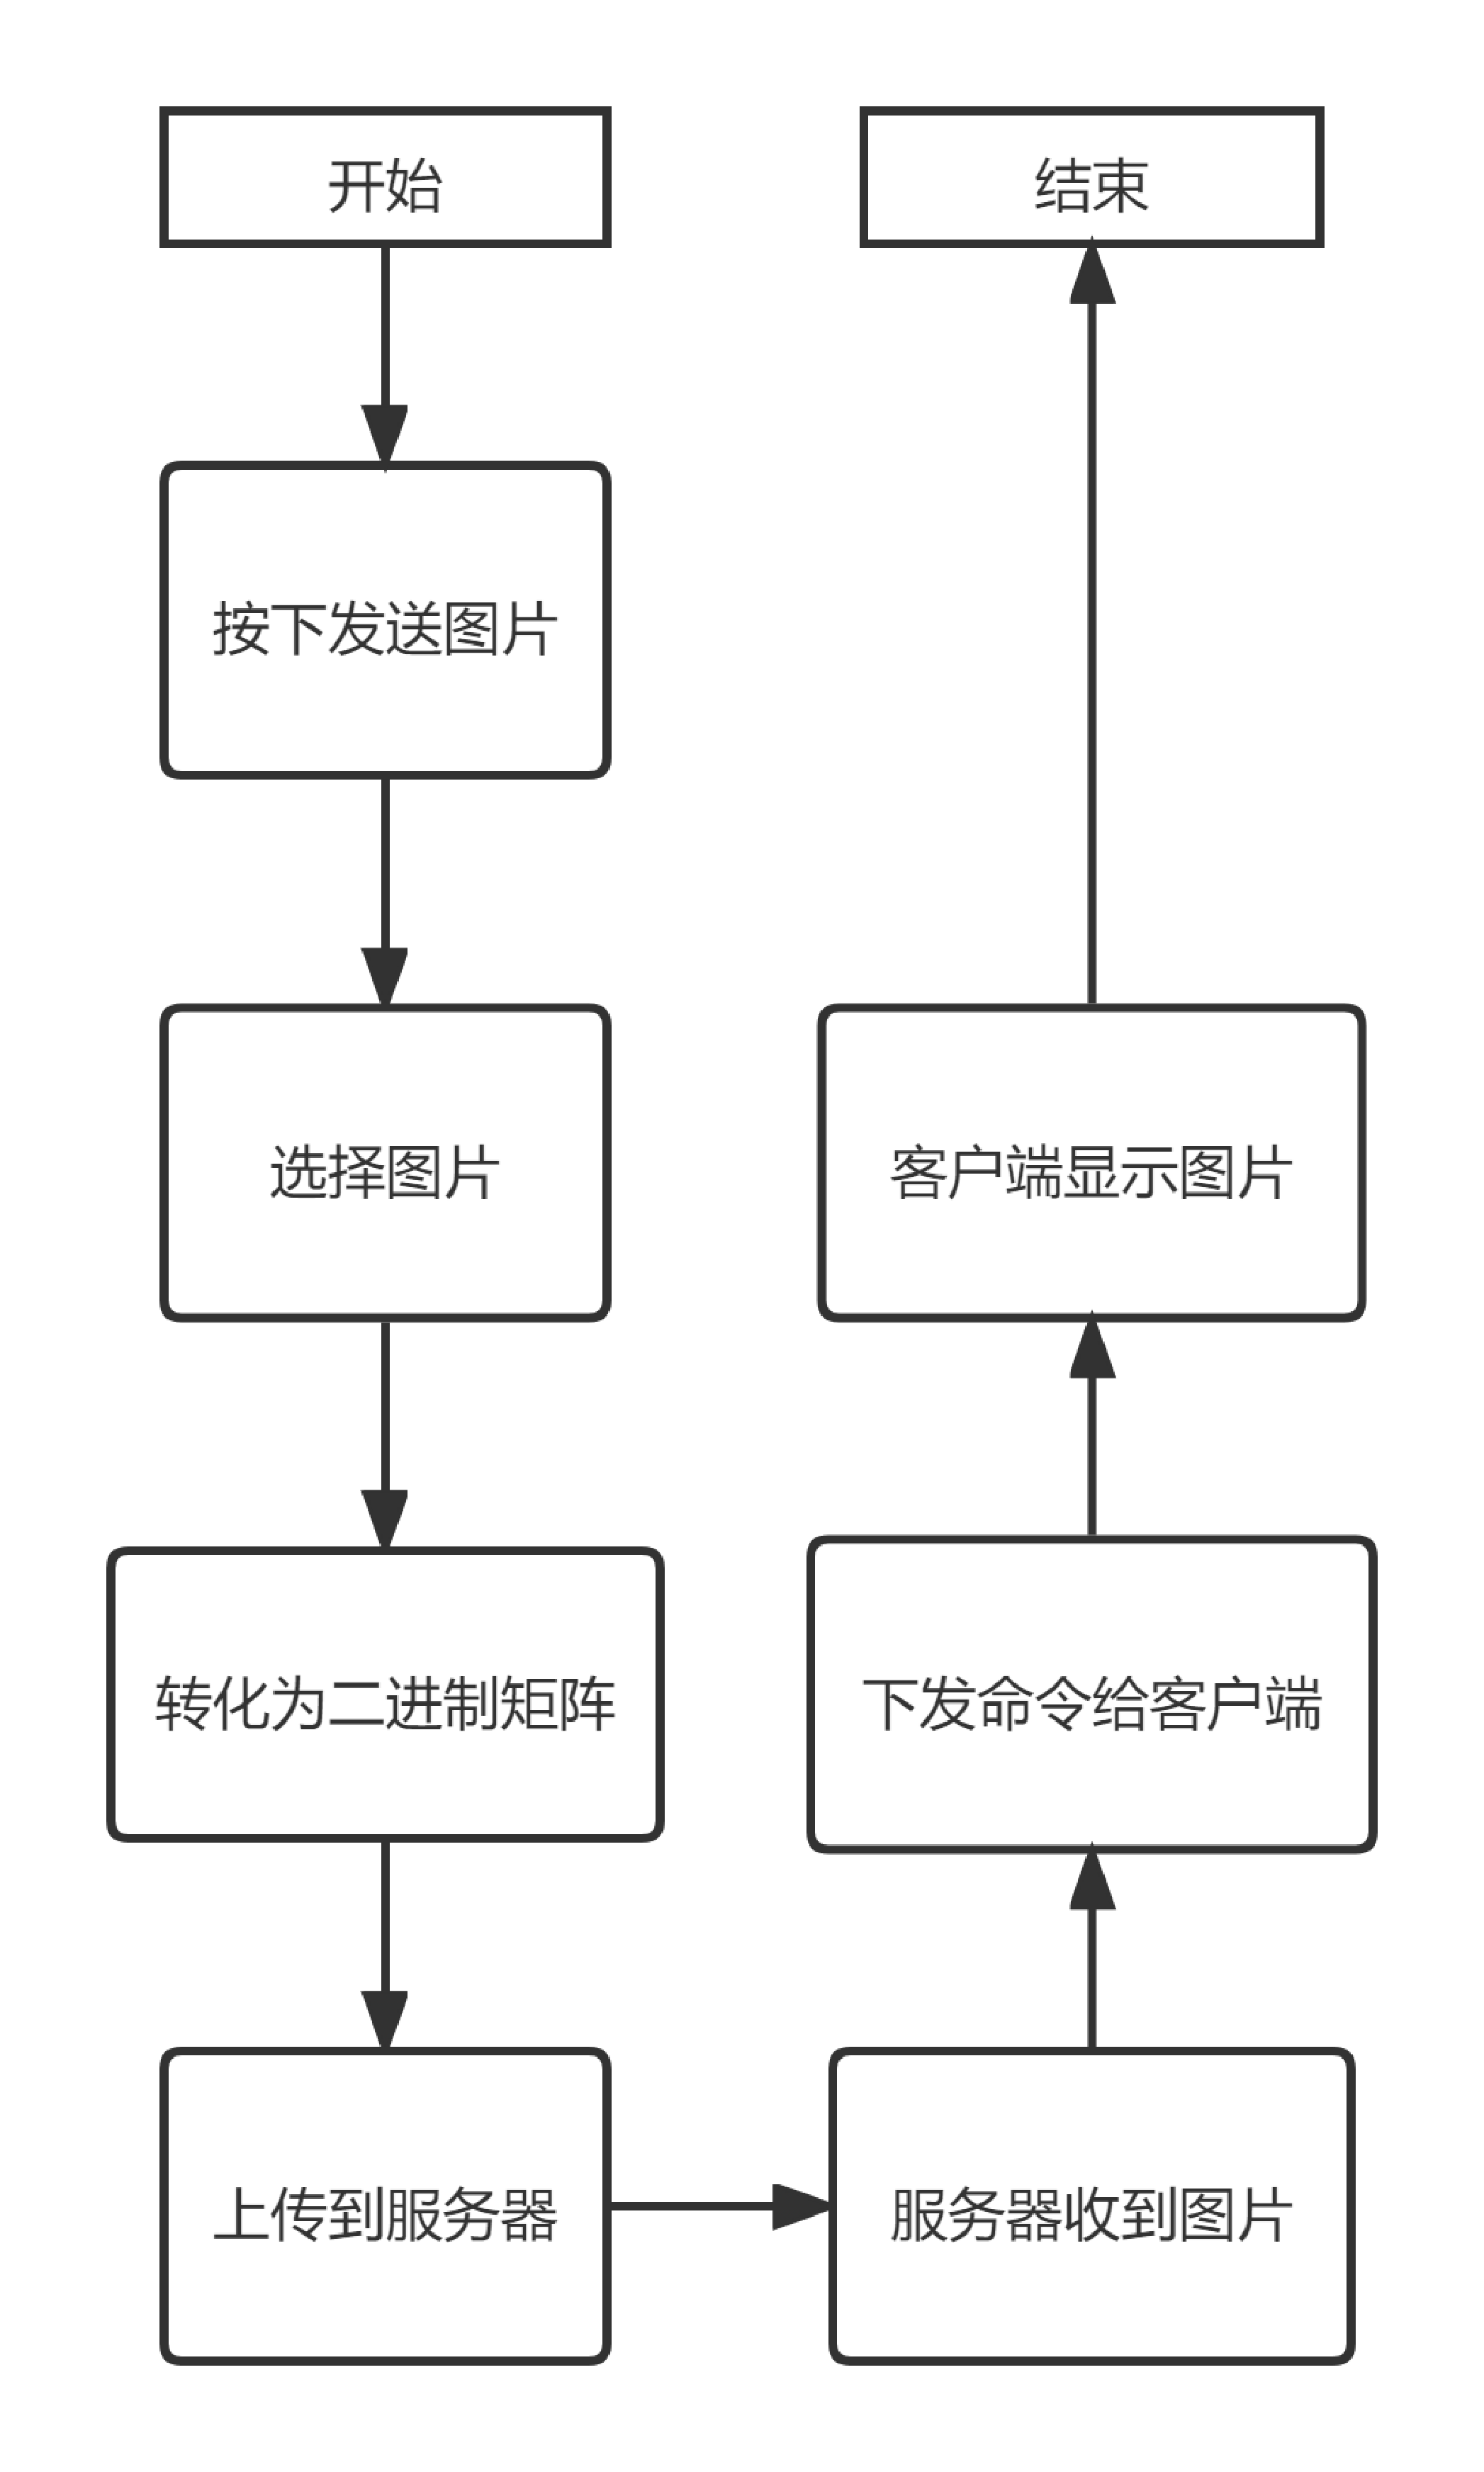
\includegraphics[width=0.3\textwidth]{picsend.pdf}
	\caption{图片收发流程图}
	\label{fig:11}
\end{figure}

选定图片,按下图片发送功能后,$opencv$ 模块将选择的图片转化为$(len,height,deep)$的矩阵形式。

$len$表示矩阵的长度。$height$表示矩阵的高度,$deep$表示图片的色域。例如$(32,32,3)$表示为一张大小为$32 \cdot 32$的彩色图片,当然,这个矩阵也可以表示为一个灰度图像;$(32,32,1)$表示为一张大小为$32 \cdot 32$的灰色图片。通过图\ref{fig:15}直观的表示了图片在计算机系统中的储存原理。

\begin{figure}[!htbp]
	\centering
	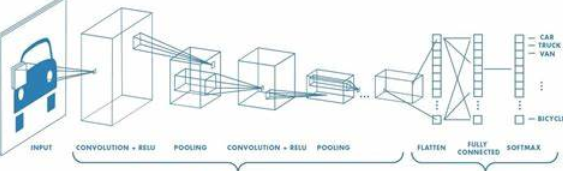
\includegraphics[width=0.6\textwidth]{picvis.png}
	\caption{矩阵图形化示意图}
	\label{fig:15}
\end{figure}

\section{消息记录}

通过使用$Neo4j$数据库实现对聊天信息的存储,当用户发送消息后,直接转发存储到数据库,流程图\ref{fig:13}展示了聊天记录保存的功能原理。

\begin{figure}[!htbp]
	\centering
	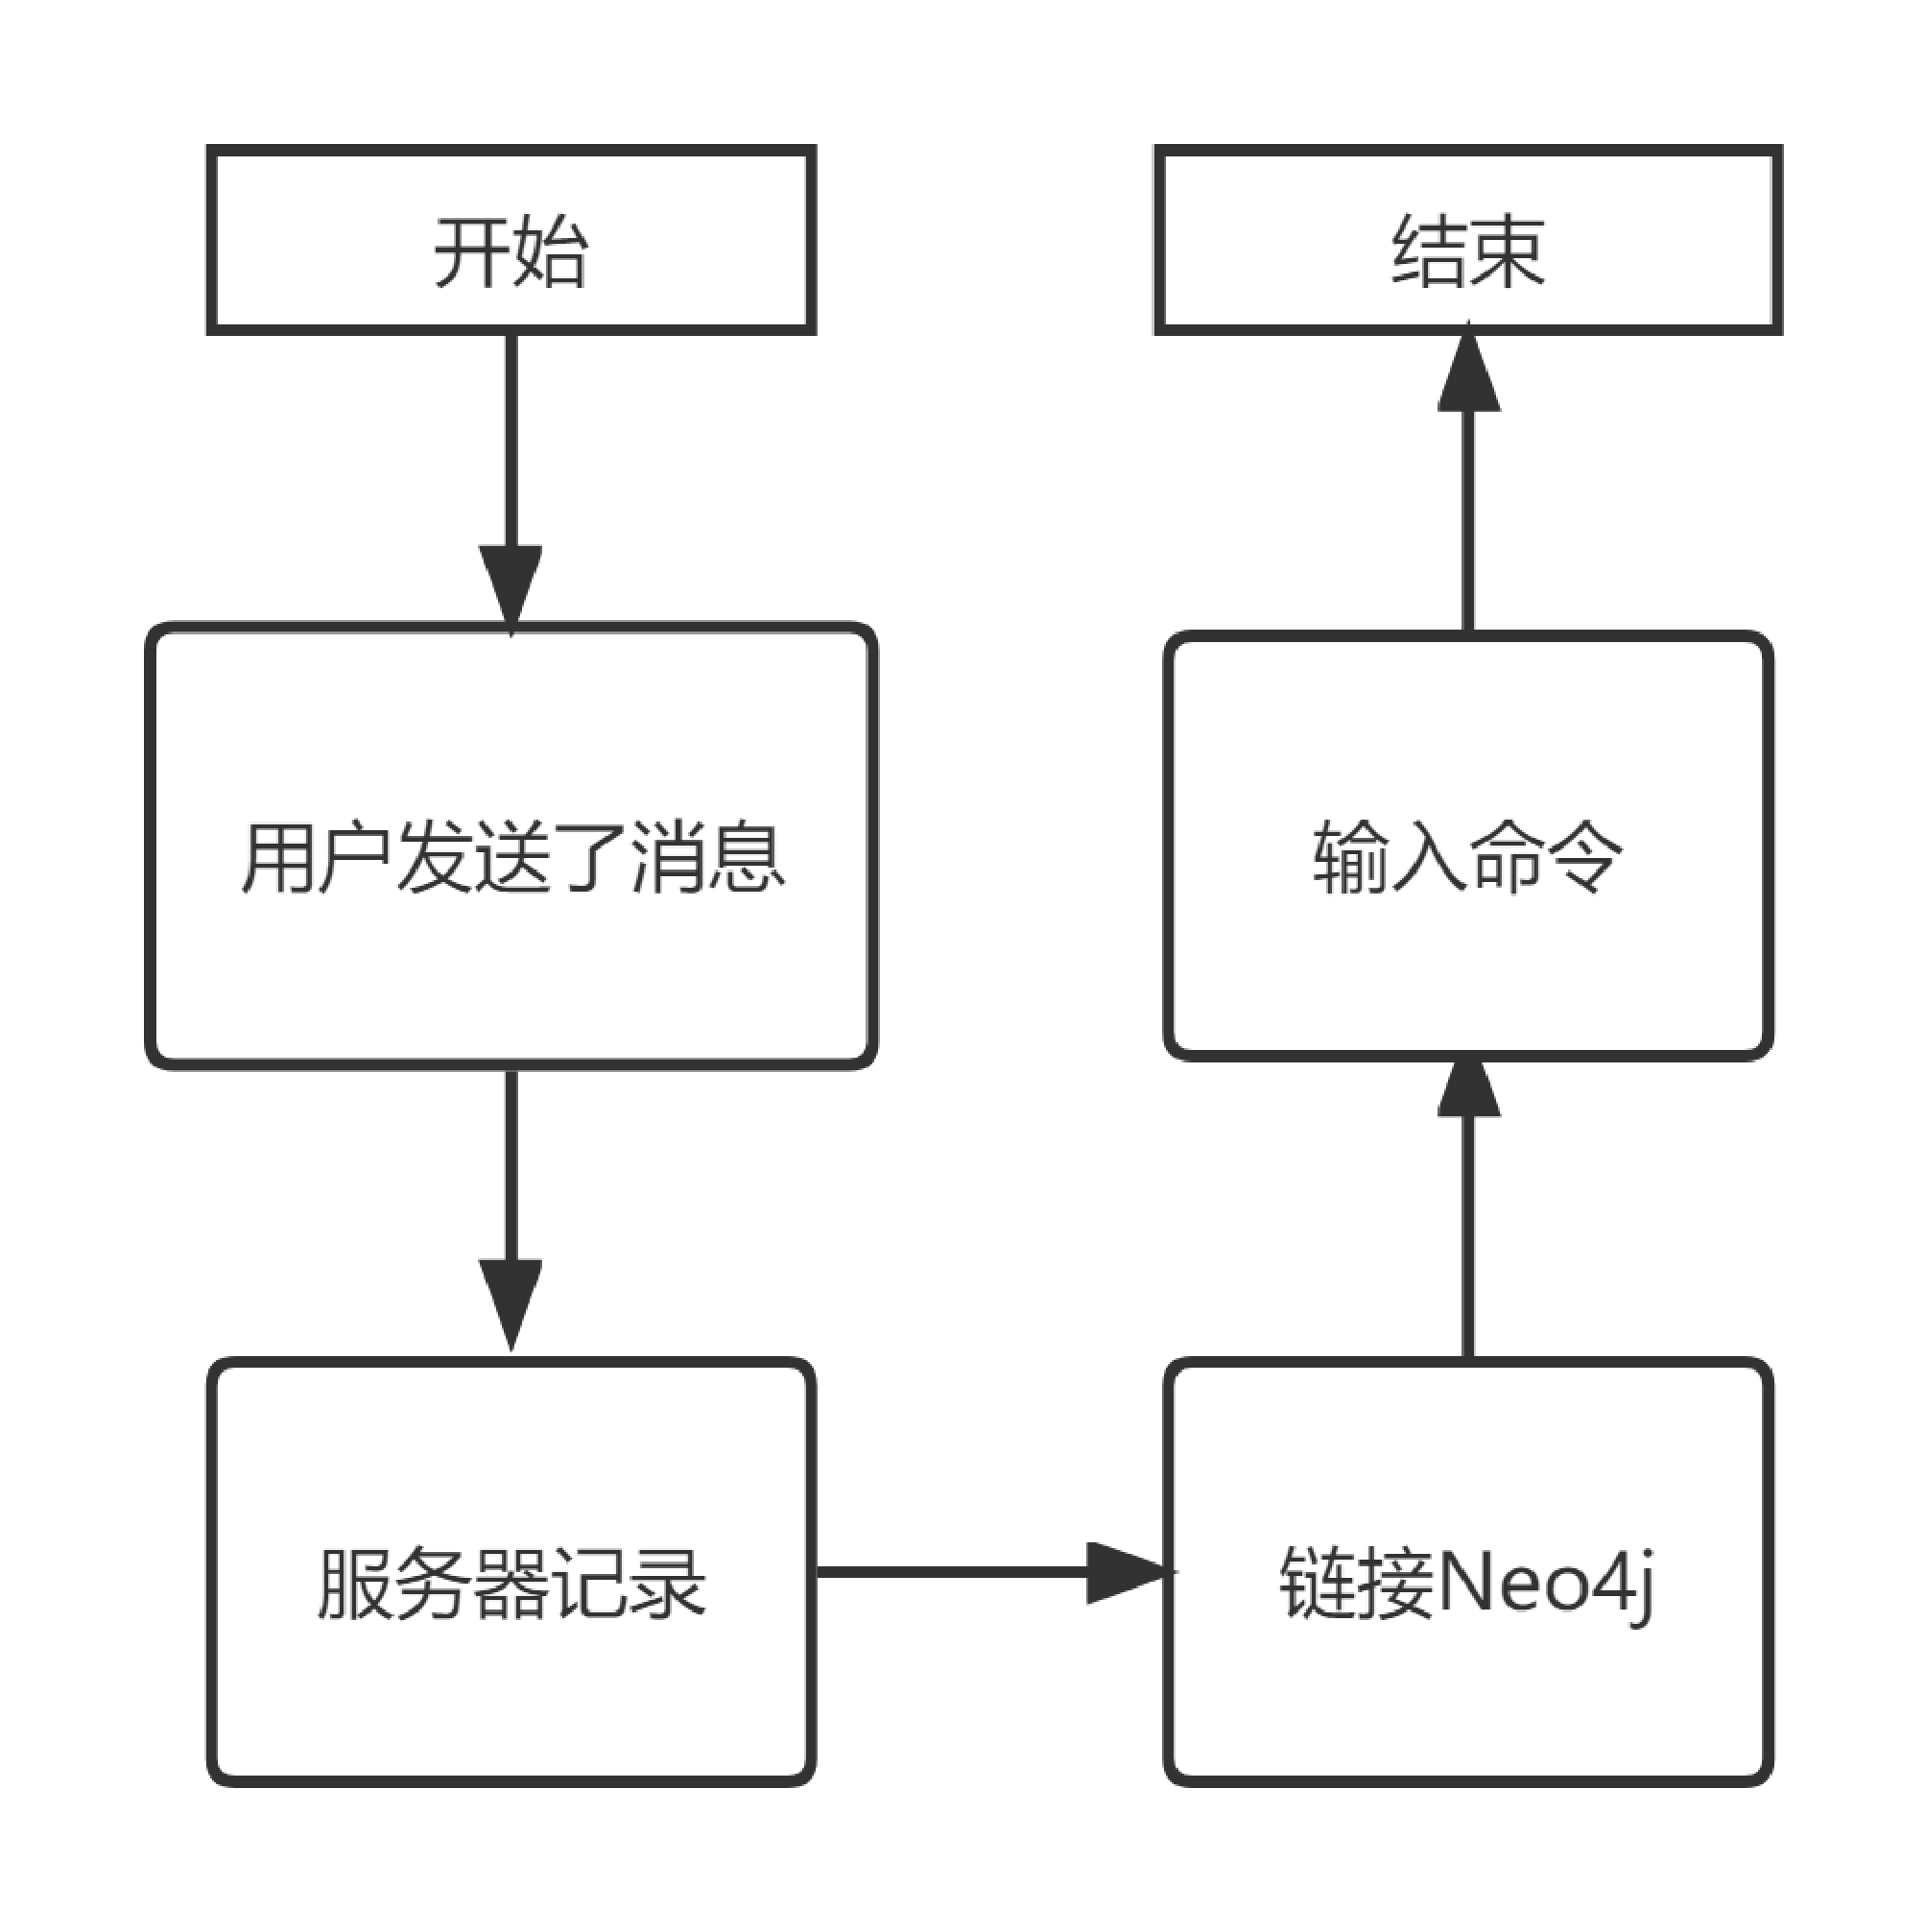
\includegraphics[width=0.3\textwidth]{mesave.pdf}
	\caption{消息保存流程图}
	\label{fig:13}
\end{figure}

首先由服务器记录下数据的形式,如果是图片,那么就把图片保存在服务器上,然后链接数据库,记录下图片保存的地址;如果是文本,就直接链接数据库,记录下文本信息。

\section{云服务器}

本软件运行在阿里云服务器,公网$IP$地址为\ref{equ:1},内网$IP$地址为\ref{equ:2}:

\begin{equation}
	\label{equ:1}
	47.100.93.63
\end{equation}
\begin{equation}
	\label{equ:2}
	172.24.12.68
\end{equation}
\clearpage
\chapter{数据结构设计}
\section{队列}

\section{文本接收}

当服务器处于高并发状态时,这时就需要使用队列了。

如图\ref{fig:12}所示,队列的工作原理遵循“先进先出”的原则,这样就可以保证先发送的消息先传输到各个用户,后发送的消息被后接受,从而确保时序的稳定。

\begin{figure}[ht]
	\centering
	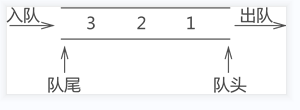
\includegraphics[width=0.5\textwidth]{duilie.png}
	\caption{队列优先}
	\label{fig:12}
\end{figure}

\section{嵌套字}

无论使用哪一种地址家族,嵌套字的类型只有两种。一种是面向连接的套接字,即:在通信之前一定要建立一条连接,就像跟朋友打电话时那样,这种通信方式也被成为“虚电路” 或 “流套字节”。面向连接的通信方式提供了顺序的、可靠的、不会重复的数据传输,而且也不会被加上数据边界。这也意味着,每一个要发送的信息,可能会被拆分成多份,每一份都会不多不少地正确到达目的地。然后被重新安顺序拼装起来,传给正在等待的应用程序。
\clearpage
\chapter{关键技术与系统实现}

\section{登录}

\subsection{功能技术}

用户在输入账号和密码以后,按下$Enter$或者登录按钮,程序将输入的字符串转化为嵌套字,传输到服务器端,服务器端启动数据库查询功能,如果用户名存在,但是密码错误,
返回-1,客户端弹出“密码错误”提示;如果用户名不存在,返回0,客户端弹出“用户名不存在”提示;如果用户名和密码都匹配,返回1,客户端弹出“登录成功”提示,跳转到聊天框。包括注册系统在内的返回值均列在了表\ref{table:3}中。

\begin{table}[ht]
	\caption{登录\&注册 返回值}
	\label{table:3}
	\begin{tabular}{ccl}
		\hline
		返回值 & 提示     & 备注                         \\ \hline
		-1  & 密码错误   & 用户输入了存在的账号,但是密码不匹配,保留该界面   \\
		0   & 用户名不存在 & 用户输入了不存在的账号,不进行密码匹配,保留该界面  \\
		1   & 登录成功   & 用户输入了匹配的账号和密码,登陆成功,跳转到聊天栏  \\
		2   & 用户名已存在 & 用户注册的账号已经存在,保留注册界面         \\
		3   & 注册成功   & 用户注册账号成功,保留注册界面录 \\
		4   & 账号或密码过短   & 用户注册账号失败,保留注册界面录 \\ \hline
	\end{tabular}
\end{table}

\subsection{实现}

其用户端的代码原理如下,通过判定返回的$receive$值,对$UI$界面发送不同的命令,提示不同的文本信息。

\begin{lstlisting}[language=Python]
if recevie == -1:
	tkinter.messagebox.showwarning('warning', message='用户名或密码不匹配')
elif receive == 0:
	tkinter.messagebox.showwarning('warning', message='用户名不存在')
elif receive == 1:
	tkinter.messagebox.showwarning('warning', message='登陆成功')
LoginUI.destroy()
\end{lstlisting} 

在服务器端,接入数据库并且进行判定账号信息的代码是:

\begin{lstlisting}[language=Python]
def isCoupleAccountPassword(g, acc, pas):
a = g.run("MATCH (n:user {" + "account:" + "\'{}\'".format(acc) + "}) RETURN n.password").data()
if not a:
	return 0
elif a[0]['n.password'] == pas:
	return 1
else:
	return -1
\end{lstlisting} 

用户登录成功后,给服务器端发送用户名,服务器端的聊天界面显示该用户已在线。

\section{注册}

\subsection{功能技术}

用户在输入账号和密码以后,按下注册按钮,和登录相同,服务器先匹配用户名是否存在,如果存在,返回2,客户端提示“用户名已存在”;否则,返回3,客户端提示”注册成功“,此时,按下登录即可使用注册的账号进行登录,返回值对于的效果见表\ref{table:3}所示。

\subsection{实现}

其用户端的代码原理如下,通过判定返回的$receive$值,对$UI$界面发送不同的命令,提示不同的文本信息。

\begin{lstlisting}[language=Python]
	if recevie == 2:
	tkinter.messagebox.showwarning('warning', message='用户名已存在')
	elif receive == 3:
	tkinter.messagebox.showwarning('warning', message='账号注册成功')
	elif receive == 4:
	tkinter.messagebox.showwarning('warning', message='账号或密码过短')
	LoginUI.destroy()
\end{lstlisting} 

在服务器端,接入数据库并且进行判定账号信息的代码是:

\begin{lstlisting}[language=Python]
def RegisterNeo4j(g, acc, pas):
	if len(acc) <=5 or len(pas)<=5:
		return 4
	elif isAccountExist(g, acc):
		return 2
	else:
		label = 'user'
		attrs = {"name": acc, "account": acc, "password": pas}
		CreateNode(g, label, attrs)
		return 3
\end{lstlisting} 

至此,账号的注册功能完成了。

\section{文本发送}

\subsection{功能技术}

当登录成功后,将显示聊天窗口,左上角部分为文本显示区域,显示别人发送的群聊、单聊文本;左下角为输入框,输入文本,其右边是发送按键,按下后即可发送;右侧是功能栏,包含发送图片、发送视频等功能。

若用户想要群聊,只需要输入文本$Text_0$,每个人都会接收到文本$Text_0$;若用户想要单聊,则在原先需要输入的 $Text_0$ 后额外输入 $ \sim $  用户名,即字符串\ref{equ:3}:
\begin{equation}
	\label{equ:3}
	Text = Text_0 + \sim + UserName
\end{equation} 

例如,“我”想要和用户“Tom”私聊,对话内容是“你今天吃饭了吗?”,那么“我”应该输入字符串\ref{equ:4}。

\begin{equation}
	\label{equ:4}
	Text = \mbox{你今天吃了吗} \sim Tom
\end{equation} 

TCP提供面向连接的可靠字节流服务。两个使用TCP的应用必须先建立TCP连接,然后客户端才能连续向服务器发送请求,如发送聊天消息、给主播送礼物、点歌等。服务器将执行一系列复杂的处理操作,并在处理完成后响应客户销。此过程花费的时间如不考虑阿络延迟可达到微秒级。\upcite{r5}
\subsection{实现}

首先,用户打开本软件后,立即接入服务器端,其中,$IP$ 和 $PORT$预先设定,为\ref{equ:1}的地址和表\ref{table:4}的端口。

\begin{lstlisting}[language=Python]
s = socket.socket(socket.AF_INET, socket.SOCK_STREAM)
s.connect((IP, int(PORT)))
\end{lstlisting} 

用户输入完需要发送的信息后,点击发送按钮后,文本被解构为\ref{equ:8}:

\begin{equation}
	Text = 0+Text_{0}+\sim+sender+\sim+receiver
	\label{equ:8}
\end{equation}

如果没有设置私聊对象,那么默认为$all$,最前面的0的作用是定义该条消息为文本类型。

\begin{lstlisting}[language=Python]
message = InputTextLabel.get() + '~' + user + '~' + chat
s.send(("0" + message).encode())
InputText.set('')
\end{lstlisting} 

在服务器端,使用多线程持续侦测是否有数据被发送,一旦收到消息,立即转发给私聊对象或者用户。

\begin{lstlisting}[language=Python]
while True:
	if not messages.empty():
	message = messages.get()
	if isSecretary(message):
		i = isSeReceiver(message)
		users[i].send(data.encode())
	else:
		for i in len(users):
			users[i].send(data.encode())
\end{lstlisting} 

\section{文本接收}

\subsection{功能技术}

客户端接收到服务器发来的信息时,首先确定是否是群发消息,如果是单发消息,那么将其颜色设置为黑色;如果是群发消息,那么将其颜色设置为红色。

在客户端接收线程中,用户循环接收服务端发来的信息(包括网名加聊天内容),将信息输出到屏幕,并清空缓冲区,为下次接收信息做准备。如果收到信息的字节数为零,则表示无数据可接收,退出客户端接收线程。\upcite{r4}

\subsection{实现}

文本接收采用$try-except$的模式。由于不同用户会在不同的时间登录,后登陆的用户可以轻易读取已经在线的用户列表,而先登录的用户要读取后进的用户信息,会显得较为复杂。本软件通过$try$功能接收信息,这样可以通过解析不同格式的$json$数据流,判断接收到的消息是添加用户还是接收文本。

为了区别文本以及后文要出现的图片、视频、文件等多种信息类型,本软件通过打包字典、发送$json$的方法将之区别开来。具体格式如表\ref{table:5}。

\begin{table}[!htbp]
	\centering
	\caption{键值对照}
	\begin{tabular}{cc}
		\hline
		键     & 值           \\
		type  & \{0,1,2,3\} \\
		value & TEXT      \\
		path  & PATH     \\ \hline
	\end{tabular}
	\label{table:5}
\end{table}

客户端界面的实现如下代码所示:
\begin{lstlisting}[language=Python]
data = s.recv(1024)
data = data.decode()
try:
	uses = json.loads(data)
	OnlineBox.delete(0, tkinter.END)
	OnlineBox.insert(tkinter.END, "当前在线用户")
	OnlineBox.insert(tkinter.END, "------Group chat-------")
	for x in range(len(uses)):
	OnlineBox.insert(tkinter.END, uses[x])
	users.append('------Group chat-------')
except:
	data = data.split('~')
	message = data[0]
	userName = data[1]
	chatwith = data[2]
            message = '\n' + message
\end{lstlisting} 

这时,接收到的数据流包含了文本和信息类型,我们通过如下代码分割出文本类型和文本。

\begin{lstlisting}[language=Python]
message = message.split(":")
message = message[0] + ":" + message[1][1:]
\end{lstlisting} 

如果$message[1][1:]$的值为0,那么这时候收到的信息就是文本,软件将文本直接显示在聊天框中。
\section{图片收发}

\subsection{功能技术}

首先使用$openCV$的$imread$功能读取图片,转化为点矩阵,再使用$FtpLib$模块连接$FTP$服务器,输入上传指令$STOR FileName$上传,输入$RETR$下载,再使用$imshow$函数显示图像,至此,完成了图片的传输和显示功能。

由于图片的读取和保存都使用$openCV$模块,这样可以确保图片的读写方式相同,避免出现$RGB565$和$RBG565$不同读取方式,提升了程序的鲁棒性。

\subsection{实现}

发送过程采用$FTP$的方式上传,同时给服务器发送一个指令,告知用户将要发送图片。

$FTP$上传的指令如下所示,通过$FTP$也可以保存下聊天记录和图片。

\begin{lstlisting}[language=Python]
file = open(FilePath, 'rb')
ftp = ftplib.FTP()
ftp.set_debuglevel(2)
ftp.set_pasv(0)
ftp.connect('47.100.93.63', 21)
ftp.login('user', '12345')
ftp.delete('test.jpg')
ftp.storbinary('STOR test.jpg', file, 1024)
ftp.close()
\end{lstlisting}

当图片发送完毕以后,给服务器发送指令$s.send(message.encode())$,其中,$message = "1" + '~' + user + '~' + chat$。服务器解析到图片即将被发送,传回客户端,先使用$FTP$功能下载图片。

\begin{lstlisting}[language=Python]
ftp = ftplib.FTP()
ftp.set_pasv(0)
ftp.connect('47.100.93.63', 21)
ftp.login('user', '12345')
filename = 'pic.jpg'
os.remove(filename)
ftp.retrbinary("RETR test.jpg", open(filename, "ab").write, 1024)
\end{lstlisting}

然后再调用$opencv$接口显示图片。

\begin{lstlisting}[language=Python]
pic = cv2.imread(filename)
cv2.imshow('picture', pic)
cv2.waitKey(0)
\end{lstlisting}

此时,接收到信息的用户界面都会显示发送者发送的图片。

\section{消息记录}

消息记录系统使用到的是数据库的查、改功能,其实现方法如下。

\subsection{存储}

消息的存储使用数据库$Neo4j$,通过建立节点存放消息,其标签分别为$sender$、$receiver$和$text$,使用$Py2neo$可以较为快速的创建一个节点,其语法如代码\ref{equ:5}。

\begin{equation}
	\label{equ:5}
	CreateRelationship(graph, label1, attrs1, label2, attrs2, name)
\end{equation}

\subsection{读取}
这时我们可以通过数据库查询代码\ref{equ:6}来获取某个发送者发送的消息,通过代码\ref{equ:7}来获取某个人接收到的消息。

\begin{equation}
	\label{equ:6}
	MATCH \; (n:sender) \; RETURN \; n:text \;
\end{equation}

\begin{equation}
	\label{equ:7}
	MATCH \; (n:receiver) \; RETURN \; n:text \;
\end{equation}

我们既可以通过$Neo4j$输入该命令,也可以在$Python$添加这个语段,输出以$Json$格式打包,可以快读在其他的数据读取程序中运行。

\section{多线程}
\subsection{优点}

由于多线程类似于同时执行多个不同程序,多线程运行有如下优点:

\begin{itemize}
	\item 使用线程可以把占据长时间的程序中的任务放到后台去处理。
	\item 用户界面可以更加吸引人,这样比如用户点击了一个按钮去触发某些事件的处理,可以弹出一个进度条来显示处理的进度
	\item 程序的运行速度可能加快
	\item 在一些等待的任务实现上如用户输入、文件读写和网络收发数据等,线程就比较有用了。在这种情况下我们可以释放一些珍贵的资源如内存占用等等。
	\item 线程可以被抢占(中断)。
	在其他线程正在运行时,线程可以暂时搁置(也称为睡眠) -- 这就是线程的退让。
\end{itemize}

\subsection{原理}

线程在执行过程中与进程还是有区别的。每个独立的进程有一个程序运行的入口、顺序执行序列和程序的出口。但是线程不能够独立执行,必须依存在应用程序中,由应用程序提供多个线程执行控制。

每个线程都有他自己的一组CPU寄存器,称为线程的上下文,该上下文反映了线程上次运行该线程的CPU寄存器的状态。

指令指针和堆栈指针寄存器是线程上下文中两个最重要的寄存器,线程总是在进程得到上下文中运行的,这些地址都用于标志拥有线程的进程地址空间中的内存。

\subsection{功能技术}

$ Python $通过两个标准库$ thread $和$ threading $提供对线程的支持。$ thread $提供了低级别的、原始的线程以及一个简单的锁。

我们将要使用的是$threating$,这个模块提供了轻量开发的便捷性,同时也保证了多线程的稳定性。

在本软件中,客户端的收发命令、收发图片、收发信息、收发视频和收发文件都用到了多线程的方法。服务器端口也同样使用了多线程,被运用在了信息发送。

一般情况下,发送者远多于接收者,那么我们就要考虑在服务器转发的过程中使用多线程,以免人数过多造成服务器卡顿。

\subsection{实现}

用发送图片来举例:

\begin{lstlisting}[language=Python]
def SendImg(*args):
	sd = threading.Thread(target=sendImg)
	sd.start()
\end{lstlisting}

$sd$是由$threating$创建的多线程窗口,传入需要进行多线程的函数名$sendImg$,这个函数就是上文发送图片的功能,那么用户在上传大文件、大视频的过程中,可以同时进行发送文本、接收消息的功能,大大方便了用户的交互体验。

\section{云服务器}

\subsection{功能使用}

配置云平台使用到了阿里云,通过阿里云的设置,可以快速创建一个较为简单的镜像。

\subsection{端口开放}

阿里云平台涉及到$Neo4j$、$FTP$等多个服务器的同时部署,在表\ref{table:4}中列出了所有需要使用到的端口。

\begin{table}[ht]
	\caption{端口及其作用}
	\label{table:4}
	\begin{tabular}{ccl}
		\hline
		端口号 & 用途     & 备注                         \\ \hline
		21  & $FTP$服务器 - $Port$ 端口   & $FTP$源文件位于C:/FTP/   \\
		80   & 服务器首页端口   & $IIS$服务提供的主页  \\
		443   & 个人网页端口   & 个人博客主页的端口  \\
		1023-1033   & $FTP$服务器 - $Passive$& 为了确保连接稳定,开启$FTP$访问模式  \\
		6666   & 网络聊天室端口   & 提供聊天室对外的端口  \\
		7474   & $Neo4j$端口 & 知识图谱数据库的对外端口        \\
		8888   & $Jupyter \; Notebook$   & $Jupyter Notebook$的对外端口 \\ \hline
	\end{tabular}
\end{table}
\clearpage

%%%=== 参考文献 ========%%%
\cleardoublepage\phantomsection
\addcontentsline{toc}{chapter}{参考文献}
\begin{thebibliography}{99}

  \bibitem{r1} 郭炳均,王思晗.网络聊天室的设计与实现[J].信息与电脑(理论版),2020,32(22):89-90.

  \bibitem{r2} 张淑坤.基于SOCKET嵌套字的IM系统设计与实现[J].数字技术与应用,2013(05):204.
  
  \bibitem{r3}温宇飞. 跨平台的聊天系统设计与实现[D].北京邮电大学,2021.
  
  \bibitem{r4}王林.基于Linux的高并发网络聊天系统设计[J].智能计算机与应用,2020,10(07):176-179.
  
  \bibitem{r5}丁乐.高并发网络服务器技术研究及在主播聊天室的应用[J].电脑编程技巧与维护,2020(07):157-158.
\end{thebibliography}

%% !Mode:: "TeX:UTF-8"
%%%%%%%%%%%%%%%%%%%%%%%%%%%%-------致谢--------%%%%%%%%%%%%%%%%%%%%%%%%%%%%%%%%

\acknowledgement
\addcontentsline{toc}{chapter}{致谢}


感谢你, 感谢他和她, 感谢大家.











 %%%致谢
\clearpage
%%%-------------- 附录. 不需要可以删除.-----------
\appendix


\chapter{代码}

\section{客户端}

\begin{lstlisting}
	import os
	import socket
	import tkinter
	import tkinter.messagebox
	import threading
	import json
	import tkinter.filedialog
	from tkinter.scrolledtext import ScrolledText
	import demo.neo4j.Neo_Fun as NeoFun
	import cv2
	import numpy as np
	import ftplib
\end{lstlisting}

\section{客户端}
\begin{lstlisting}
	import os
	import socket
	import tkinter
	import tkinter.messagebox
	import threading
	import json
	import tkinter.filedialog
	from tkinter.scrolledtext import ScrolledText
	import demo.neo4j.Neo_Fun as NeoFun
	import cv2
	import numpy as np
	import ftplib
\end{lstlisting}
\end{document}



